\chapter{Esperimenti}\label{ch:exp}
\section{Specifiche hardware e software}
Gli esperimenti sono stati condotti tramite connessione ssh ad un server del laboratorio \textit{LESC - Signal Processing \& Communications LAB} dell'Università degli Studi di Firenze; la macchina utilizzata presenta le seguenti caratteristiche:
\begin{itemize}
    \item \text{CPU}: Intel Core i9-9940X @ 3.30GHz, architettura x86\_64
    \item \text{RAM}: 125 GB
    \item \text{GPU}: 2 NVIDIA GeForce RTX 2080 Ti
    \item \text{Sistema Operativo}: Ubuntu 22.04.5 LTS (Jammy)
\end{itemize}
Le GPU presenti sono state fondamentali per svolgere l'estrazione delle rappresentazioni latenti delle immagini tramite l'uso dell'encoder neurale di JPEG AI in tempi rapidi, mentre l'addestramento e valutazione dei modelli di classificazione sono stati completamente svolti sulle CPU disponibili.
\section{Codice sorgente del lavoro}
Il codice sorgente sviluppato è reso disponibile tramite GitHub all'indirizzo \url{https://github.com/edorustichini/thesis.git}. L'intero progetto è sviluppato in Python, e nella cartella \texttt{src} sono presenti gli script per il setup degli esperimenti, metodi per processare i dati, e script per l'addestramento e valutazione dei modelli. Sono inoltre presenti dei notebook Jupyter per l'analisi dei risultati.\\
L'estrazione delle rappresentazioni latenti delle immagini viene fatta utilizzando il software  ufficiale di riferimento di JPEG AI, disponibile all'indirizzo \url{https://gitlab.com/wg1/jpeg-ai/jpeg-ai-reference-software}.
\section{Esperimenti condotti}\label{sec:experiments}
Come dichiarato nelle sezioni precedenti, l'obbiettivo del lavoro consiste nel verificare l'efficacia della codifica JPEG AI nel compito di identificazione di immagini generate.\\
Gli esperimenti sono stati condotti per ogni classificatore scelto variando 3 fattori principali:  metodo di preprocessing delle feature estratte, componente scelta e diversi bpp. Nella tabella \ref{tab:experimentalfactors} è riportato un riepilogo dei fattori considerati.
\begin{table}[H]
\centering
\caption{Fattori considerati durante gli esperimenti}\label{tab:experimentalfactors}
\begin{tabularx}{\textwidth}{l X}
\toprule
\textbf{Fattore} & \textbf{Valori / Descrizione} \\
\midrule
Compressione (Bpp) & 12bpp, 6bpp. Usati per capire l'effetto del livello di compressione sui risultati \\
\midrule
Componente target & Y e YUV \\
& - Y: classificatori allenati esclusivamente sulla componente della luminanza. \\
& - YUV: classificatori allenati su tutte e tre le componenti (Y, U, V) concatenandole. \\
\midrule
Preprocessing & Come descritto in \ref{sec:preprocessing} sono stati esplorati diversi metodi di preprocessing dei latenti prima dell'addestramento: Flatten, Single Patch e Multiple Patches. \\
\bottomrule
\end{tabularx}
\end{table}
Il metodo di preprocessing delle feature influenza la struttura del dataset di addestramento e le modalità di valutazione del modello. Nella tabella \ref{tab:preprocessing_methods} viene proposta una schematizzazione dei metodi.
\begin{table}[H]
\centering
\caption{Confronto tra metodi di preprocessing delle feature.}\label{tab:preprocessing_methods}
\begin{tabularx}{\textwidth}{l c c}
\toprule
\textbf{Method} & \textbf{Samples per Image} & \textbf{Feature Dimension} \\
\midrule
Flatten Latents (Y)        & 1 & $C_y \cdot H \cdot W = 40960$ \\
Flatten Latents (YUV)     & 1 & $(C_y +C_{uv})\cdot H \cdot W = 65536$ \\
Single Patch (Y)        & 1 & $C_y = 160$ \\
Single Patch (YUV)     & 1 & $C_y + C_{uv} = 256$ \\
N Patches (Y)    & N & $C_y = 160$ \\
N Patches (YUV)        & N & $C_y + C_{uv} = 256$ \\
\bottomrule
\end{tabularx}
\small{Nota: $H,W$ sono le dimensioni di ogni canale latente, $C_y, C_{uv}$ sono il numero di canali della componente Y e delle componenti U e V rispettivamente.}
\end{table}
\paragraph{Nota sul metodo N Patches}
Per il metodo N Patches, la fase di testing viene svolta in maniera differente rispetto alle altre: nella fase di addestramento, per ogni immagine vengono estratte N patches ottenendo un insieme di addestramento di cardinalità ($N\cdot |\mathcal{D}|$) (dove $\mathcal{D}$ è il dataset originale). Per la fase di testing invece si utilizza la strategia di \textit{majority voting}: per ogni immagine vengono estratte tutte le patch, ed il classificatore produce una predizione indipendente su ognuna di queste. La predizione finale sarà la classe più frequente tra tutte le votazioni.\\
\subsection{Metodo di addestramento}
Come descritto nella sez. \ref{subsec:tuning}, per ogni esperimento è stato svolto il tuning degli iperparametri: inizialmente è stata applicata una ricerca casuale su un intervallo di valori ampio e osservando i risultati ottenuti, è stata svolta una ricerca a griglia ristretta sui migliori 3 valori trovati per ogni iperparametro. Questo procedimento è stato ripetuto a dimensioni diverse ($15.000, 30.000, 50.000$) del dataset di addestramento, e i valori migliori sono stati usati per allenare il modello finale su $30.000$ immagini, e poi valutarlo su $3.000$ immagini di test.
La libreria scelta per gli algoritmi di machine learning è Scikit-learn, libreria open-source scritta in Python, che offre strumenti semplici ma efficienti per molte task, tra cui quelle di classificazione.
In particolare, per Random Forest e Gradient Boosting sono stati scelti i modelli nominati \texttt{RandomForestClassifier} e \texttt{HistGradientBoostingClassifier}; mentre per gli algoritmi di ricerca degli iperparametri sono stati usati \texttt{RandomizedSearchCV} e \texttt{GridSearchCV}.
%PIPELINE ADDESTRAMENTO
%\paragraph{Metriche di valutazione}
%\subsection{Metriche di valutazione per testing}
% Accuratezza, Precision, Recall, F1-Score, Confusion Matrix
%\textit{Lista di metriche usate per valutazione nei test}
%\textit{Lista degli esperimenti condotti: bpp, num samples, metodo di estrazione, Y+UV, iperparametri}
%TODO: VEDI ESEMPI DI IPERPARAMETRI https://www.ibm.com/it-it/think/topics/hyperparameter-tuning
\section{Risultati}
I risultati verrano presentati in sezioni separate per tipo di classificatore, e per ognuno vengono mostrate le varie combinazioni dei fattori descritti nella sez. \ref{sec:experiments}, presentando prima una tabella con i risultati per quel modello, e poi diagrammi a barre per la visuallizzazione.
Infine verrà fatto un confronto tra le prestazioni dei due classificatori.
\subsection{Risultati RandomForest}
Al termine del tuning degli iperparametri, la combinazione che ha avuto un \texttt{cv-score} più alto è:
\begin{lstlisting}[style=pythonElegant, caption={Miglior combinazione di parametri per RandomForestClassifier} ]
RandomForest(random_state=42, oob_score=True,
n_estimators=463, max_depth=30, max_features='sqrt',min_samples_leaf=2)
\end{lstlisting}
Nella tabella \ref{tab:RF-results-table} sono riportati i risultati sull'accuratezza ottenuti dal modello scelto negli esperimenti. 
\begin{table}[H]
\centering
\caption{Risultati per Random Forest}\label{tab:RF-results-table}
\begin{tabular}{lrllrr}
\toprule
Modello &  Bpp &  Comp. &     process. &     $y$ &  $\hat{y}$ \\
\midrule
RF &  6 &       Y &   single & 0.683 &  0.683 \\
RF &  6 &       Y & multiple & 0.607 &  0.597 \\
RF &  6 &       Y & flatten & 0.801 & 0.789  \\
RF & 12 &       Y &   single & 0.683 &  0.682 \\
RF & 12 &       Y & multiple & 0.568 &  0.560 \\
RF &  12 &       Y & flatten &  0.807&  0.801\\

\midrule
RF &  6 &     YUV &  flatten & 0.820 &  0.811 \\
RF &  6 &     YUV &   single & 0.720 &  0.716 \\
RF &  6 &     YUV & multiple & 0.630 &  0.605 \\
RF & 12 &     YUV &  flatten & 0.824 &  0.804 \\
RF & 12 &     YUV &   single & 0.720 &  0.718 \\
RF & 12 &     YUV & multiple & 0.650 &  0.632 \\
\bottomrule
\end{tabular}
\end{table}
\begin{figure}[H]
    \centering
    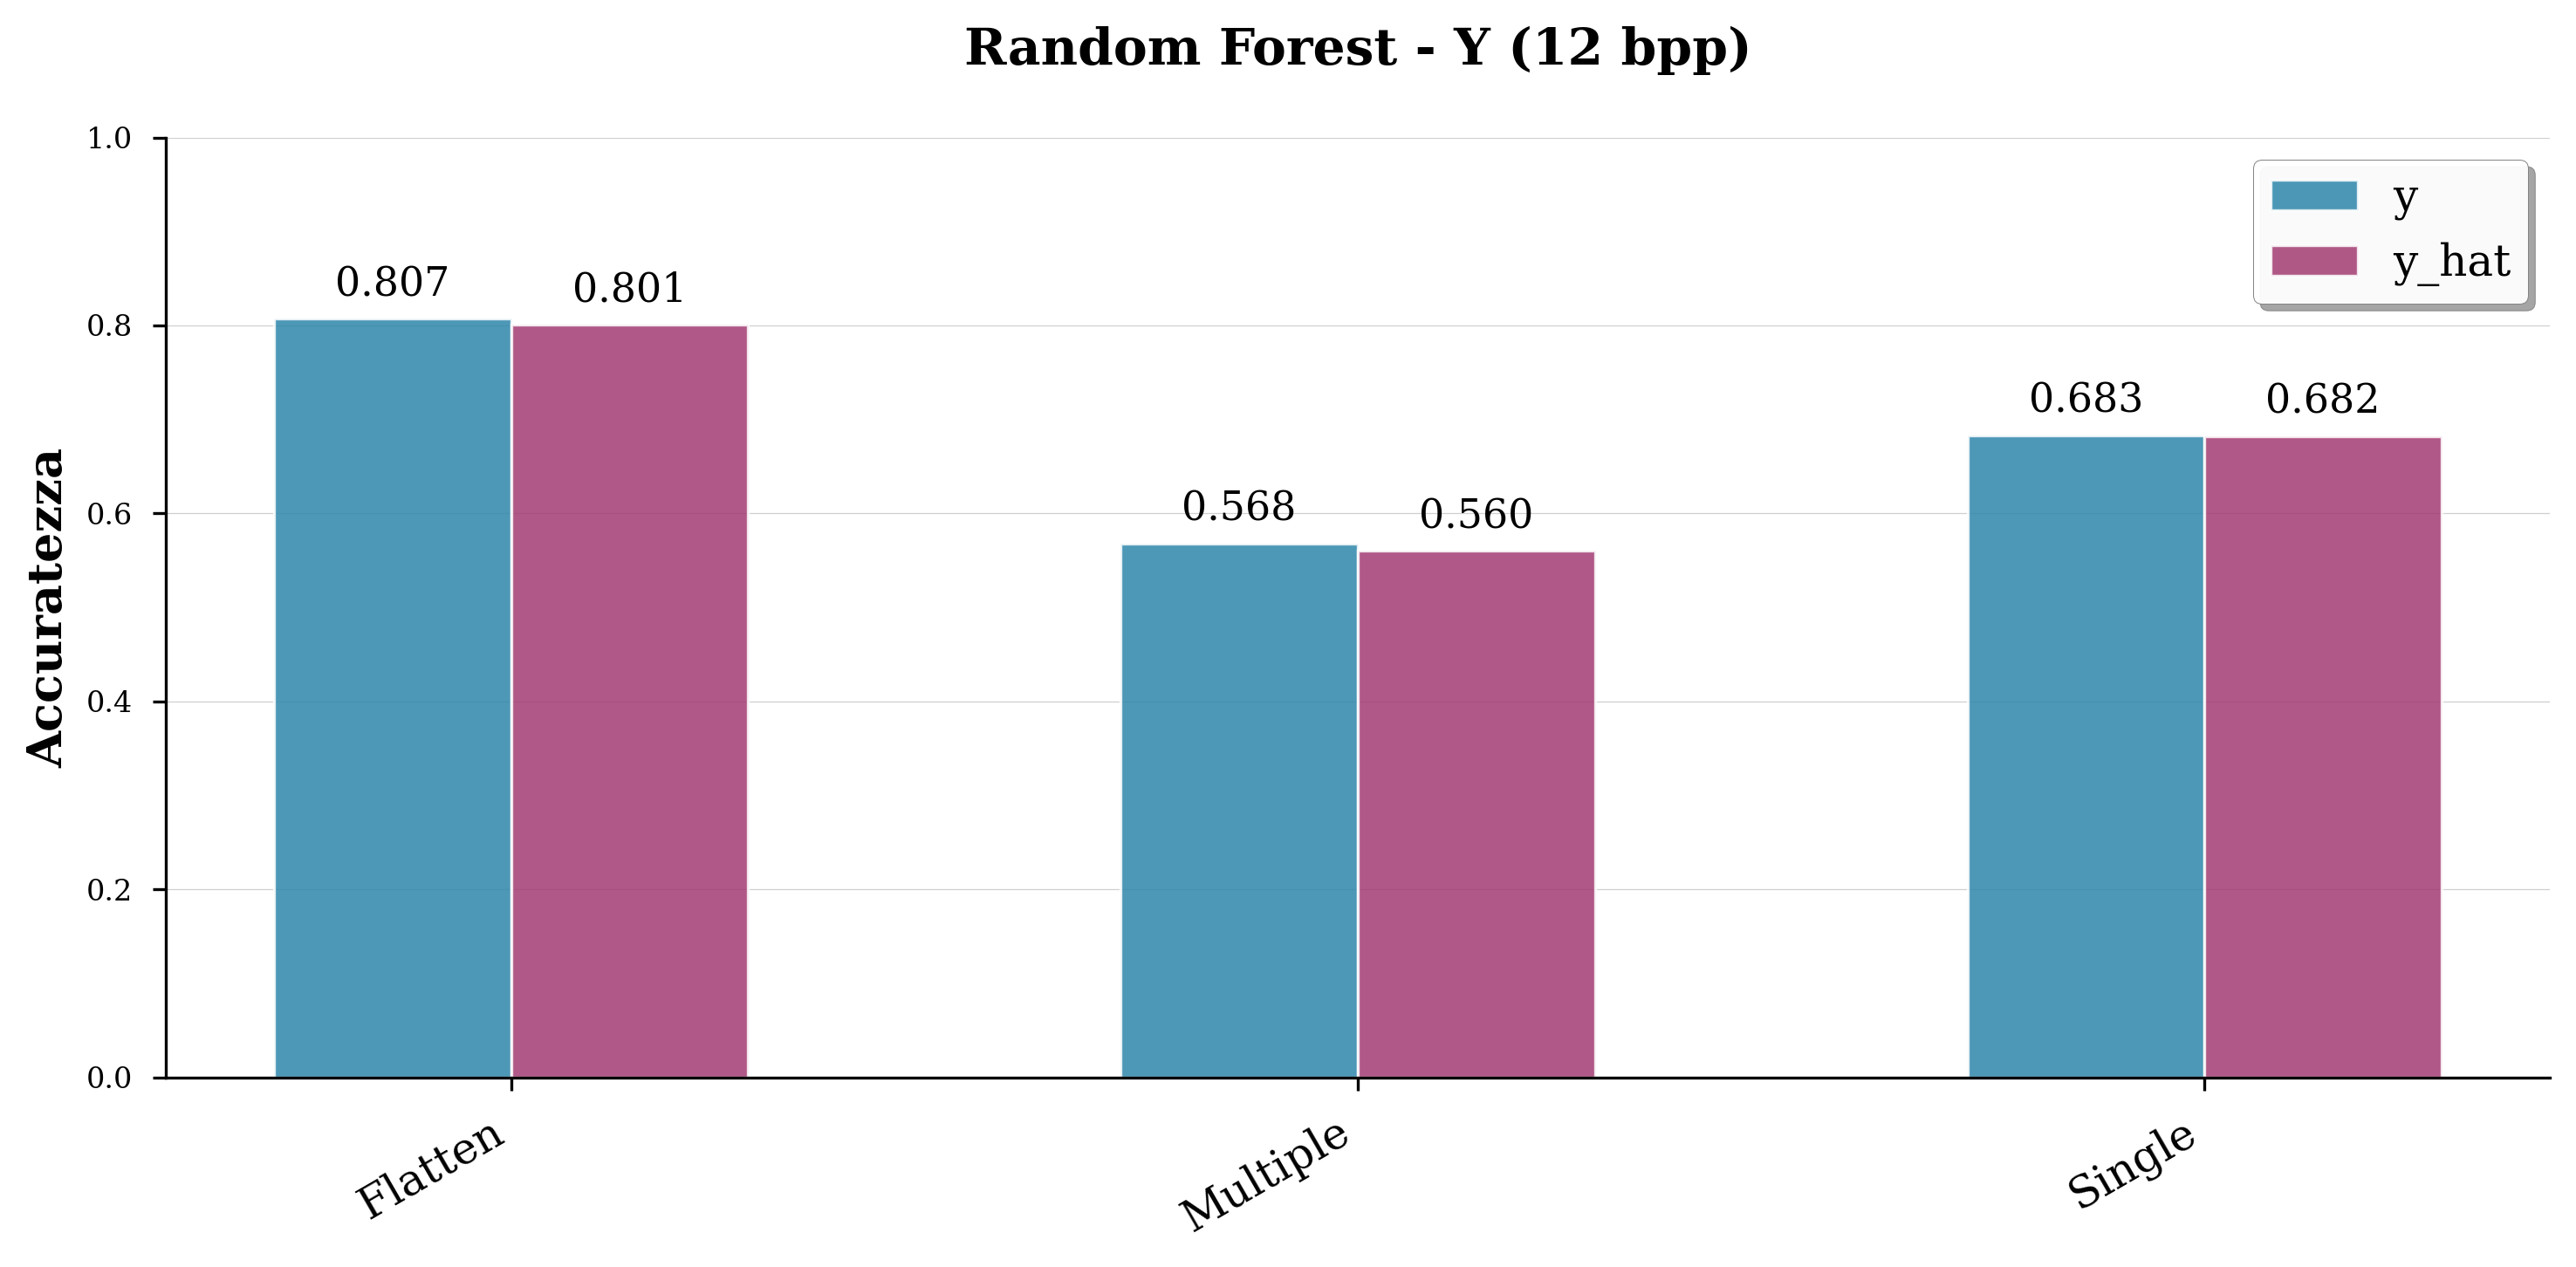
\includegraphics[width=0.8\textwidth]{figures/RF_Y_12bpp_improved.png}\\[0.5cm]
    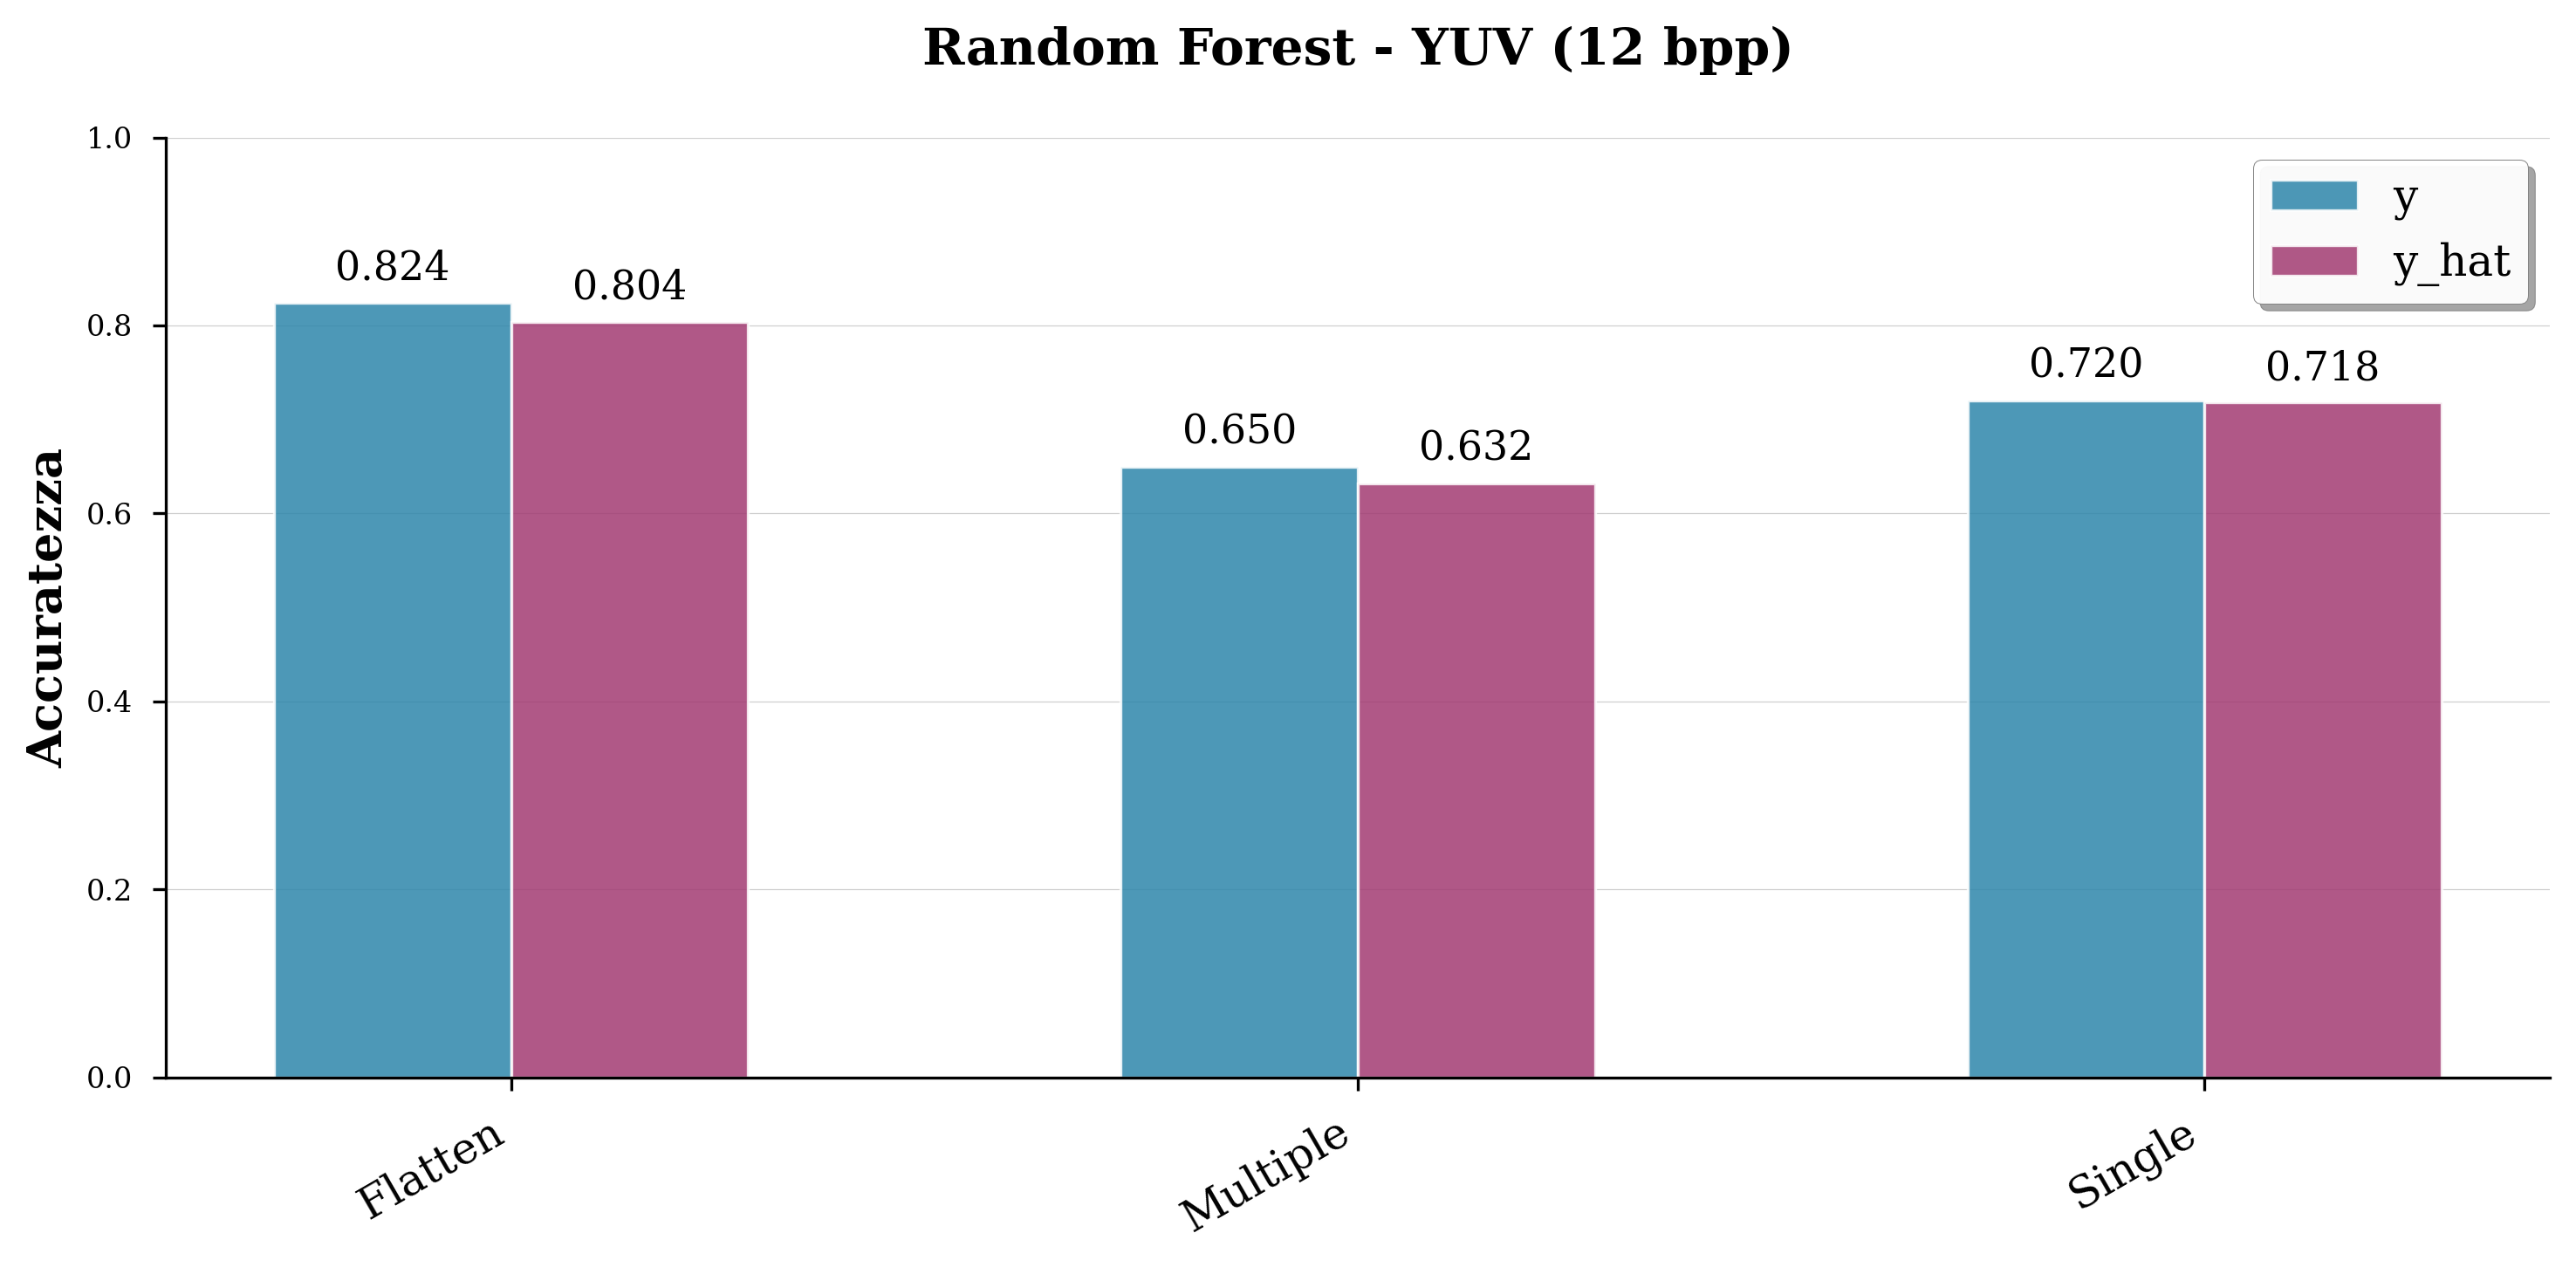
\includegraphics[width=0.8\textwidth]{figures/RF_YUV_12bpp_improved.png}
    \caption{Confronto tra prestazioni di due Random Forest allenati Y e YUV.}
    \label{fig:RF_YvsYUV}
\end{figure}
Dalla figura \ref{fig:RF_YvsYUV} si nota come le prestazioni del Random Forest allenato su YUV siano  migliori rispetto a quello allenato solo su Y, in particolare nel caso del metodo di processing "single patch".
Nella figura \ref{fig:RF_YUV_confusion} sono riportate le matrici di confusione per le configurazioni che hanno ottenuto migliori prestazioni con l'uso di Random Forest.
\begin{figure}[H]
    \centering
    \begin{subfigure}[b]{0.7\textwidth}
        \centering
        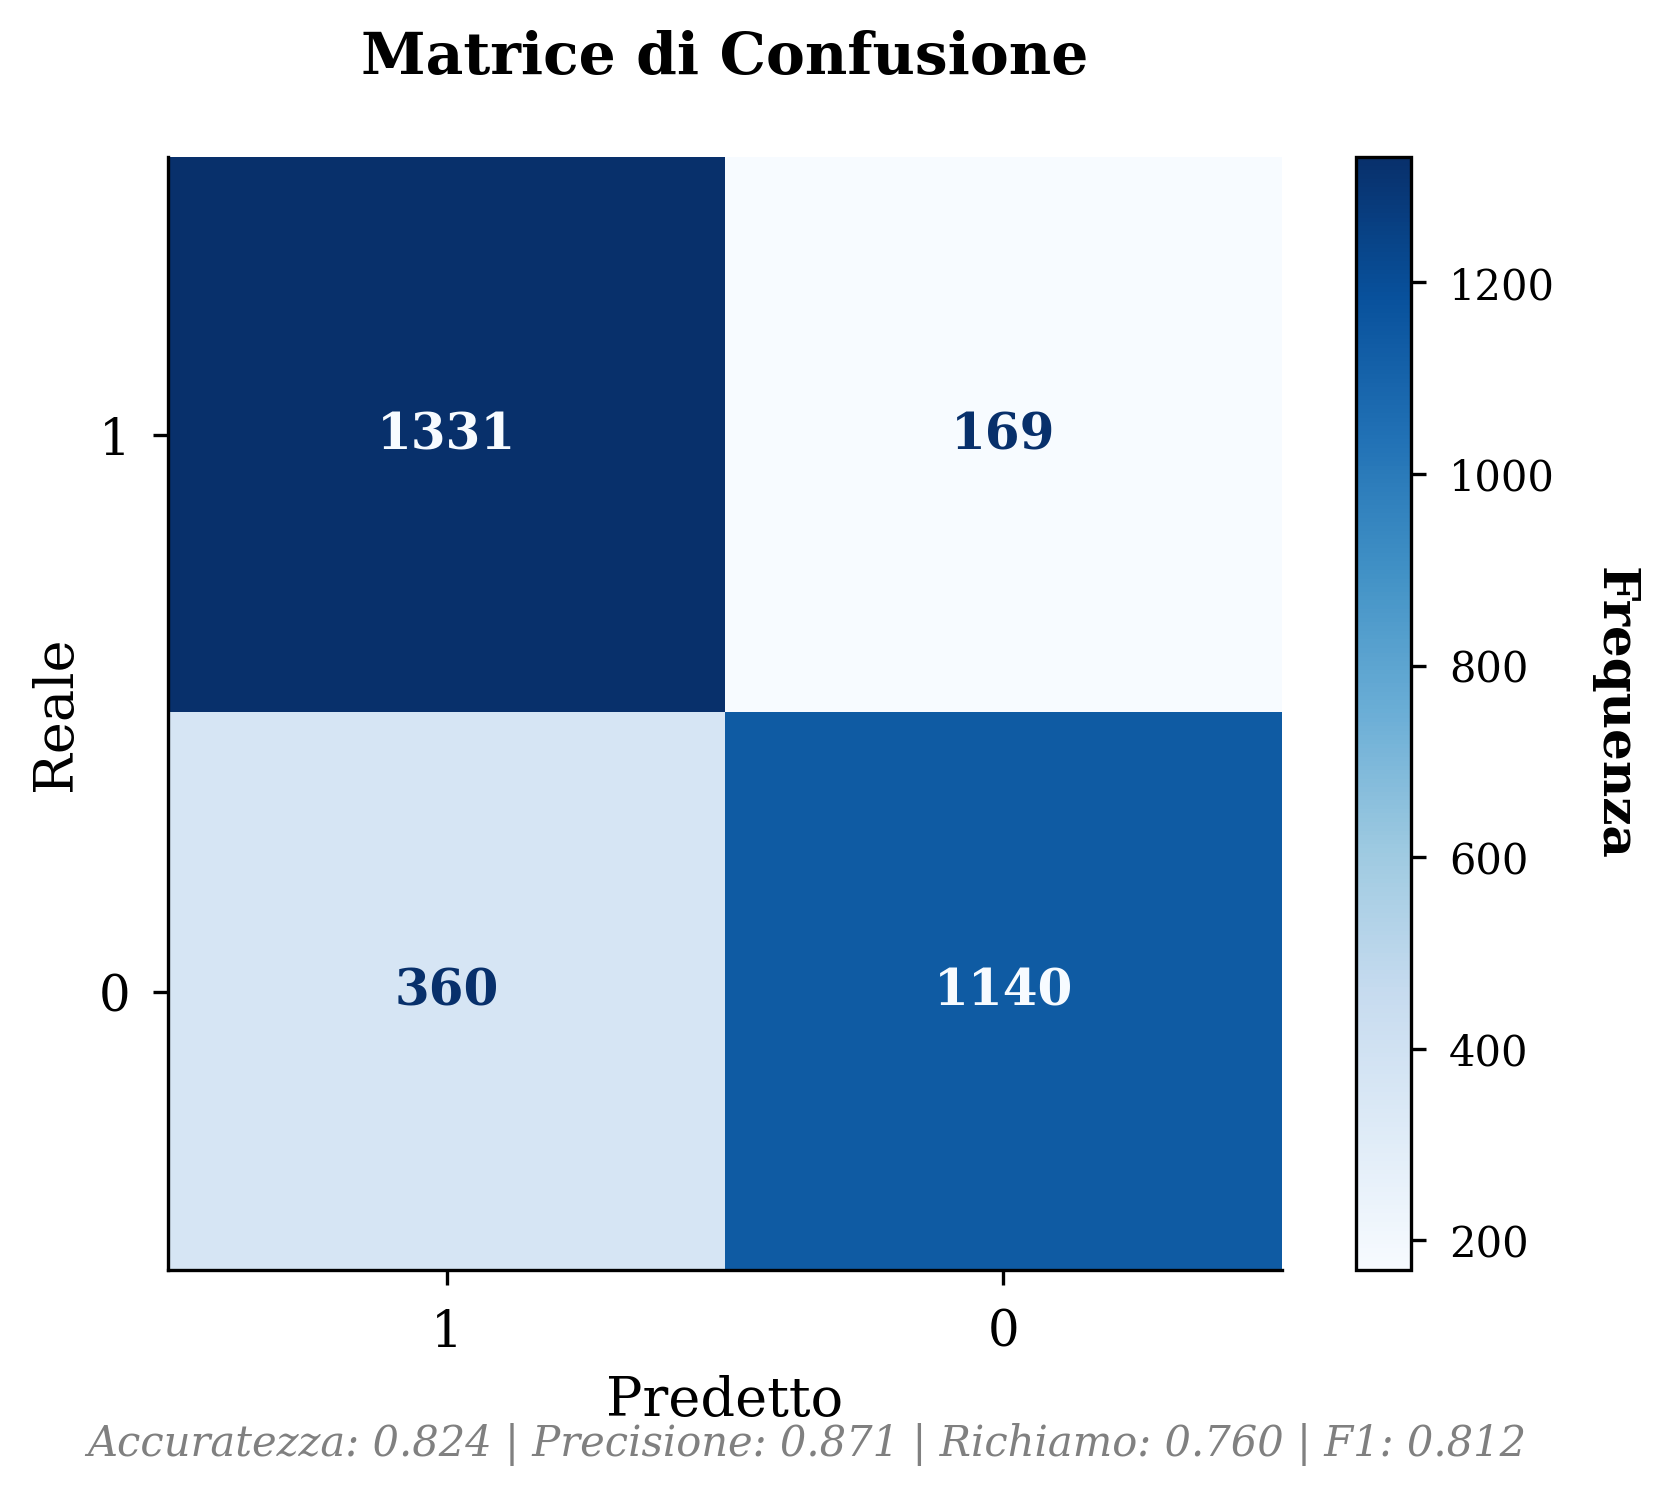
\includegraphics[width=\textwidth]{figures/confusion_matrix_flatten_YUV_RF.png}
        \caption{Metodo flatten}
    \end{subfigure}
    \hfill
    \begin{subfigure}[b]{0.7\textwidth}
        \centering
        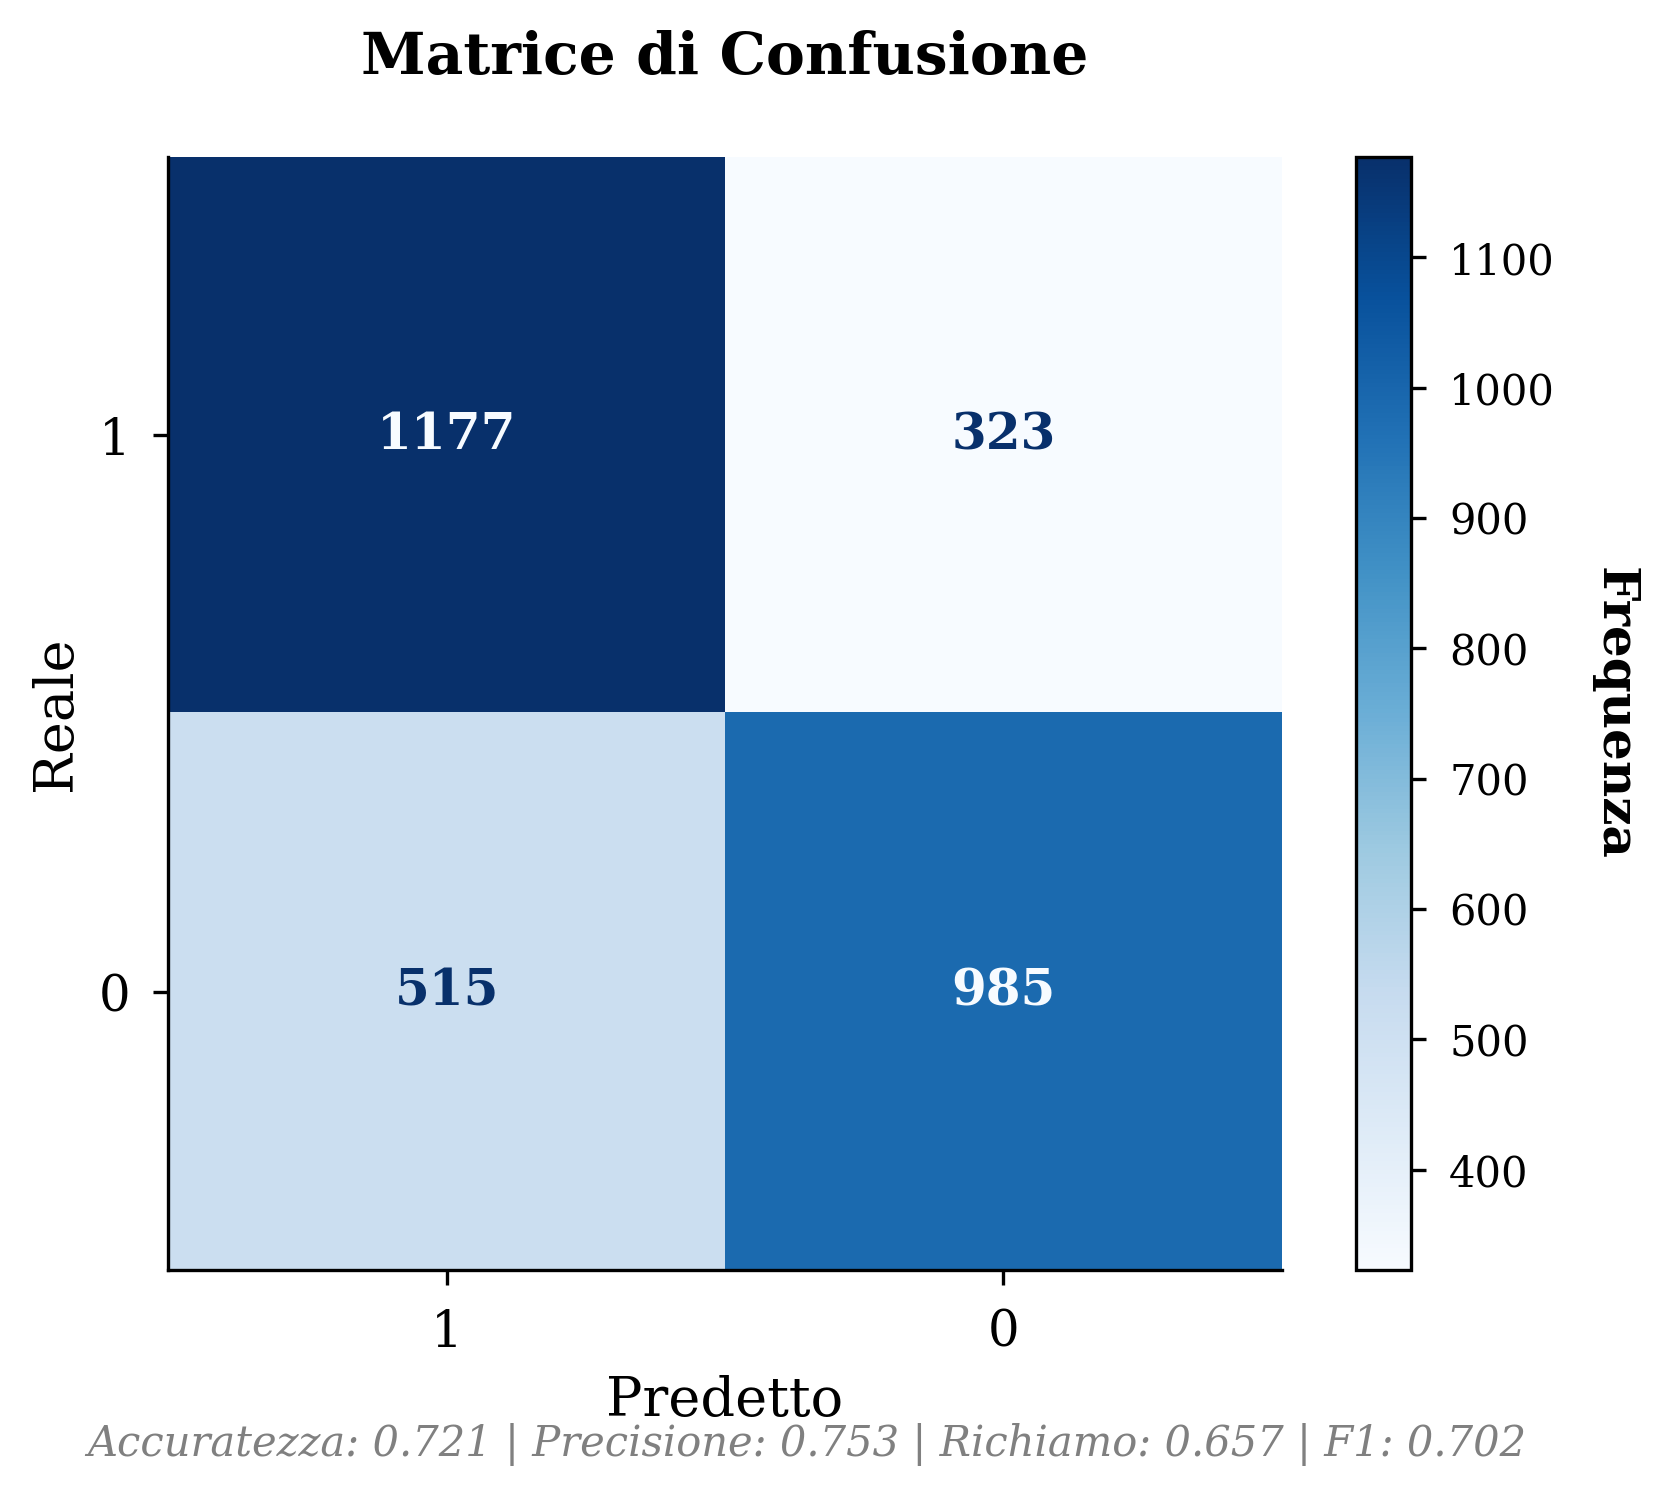
\includegraphics[width=\textwidth]{figures/confusion_matrix_YUV_single_RF.png}
        \caption{Metodo single patch}
    \end{subfigure}
    \caption{Matrici di confusione per Random Forest allenato su YUV con due approcci diversi.}
    \label{fig:RF_YUV_confusion}
\end{figure}

\subsection{GradientBoosting}
La combinazione migliore di iperparametri trovata per l'algoritmo di Gradient Boosting è:
\begin{lstlisting}[style=pythonElegant]
    GradientBoostingClassifier(
        learning_rate=0.12965912630431367,
        max_iter=596,
        max_leaf_nodes=117,
        min_samples_leaf=18,
        l2_regularization=0.003042734607209594,
        random_state=42,
        validation_fraction=0.1)
\end{lstlisting}
Come fatto per il Random Forest, nella tabella (\ref{tab:GB-results-table}) sono riportati tutti i risultati ottenuti da Gradient Boosting.
\begin{table}[H]
\centering
\caption{Risultati per Gradient Boosting}
\label{tab:GB-results-table}
\begin{tabular}{lrllrr}
\toprule
Modello &  Bpp &  Comp. &     process. &     $y$ &  $\hat{y}$ \\
\midrule
GB &  6 &       Y &   single & 0.696 &  0.688 \\
GB &  6 &       Y & multiple & 0.543 &  0.535 \\
GB &  6 &       Y & flatten & 0.890 & 0.870 \\
GB & 12 &       Y &   single & 0.695 &  0.700 \\
GB & 12 &       Y & multiple & 0.554 &  0.534 \\
GB & 12 &       Y & flatten & 0.900 & 0.890 \\
\midrule
GB &  6 &     YUV &   single & 0.744 &  0.753 \\
GB &  6 &     YUV & multiple & 0.670 &  0.645 \\
GB &  6 &     YUV &  flatten & 0.940 &  0.940 \\
GB & 12 &     YUV &   single & 0.744 &  0.744 \\
GB & 12 &     YUV & multiple & 0.680 &  0.667 \\
GB & 12 &     YUV &  flatten & 0.944 &  0.940 \\
\bottomrule
\end{tabular}
\end{table}
\begin{figure}[H]
    \centering
    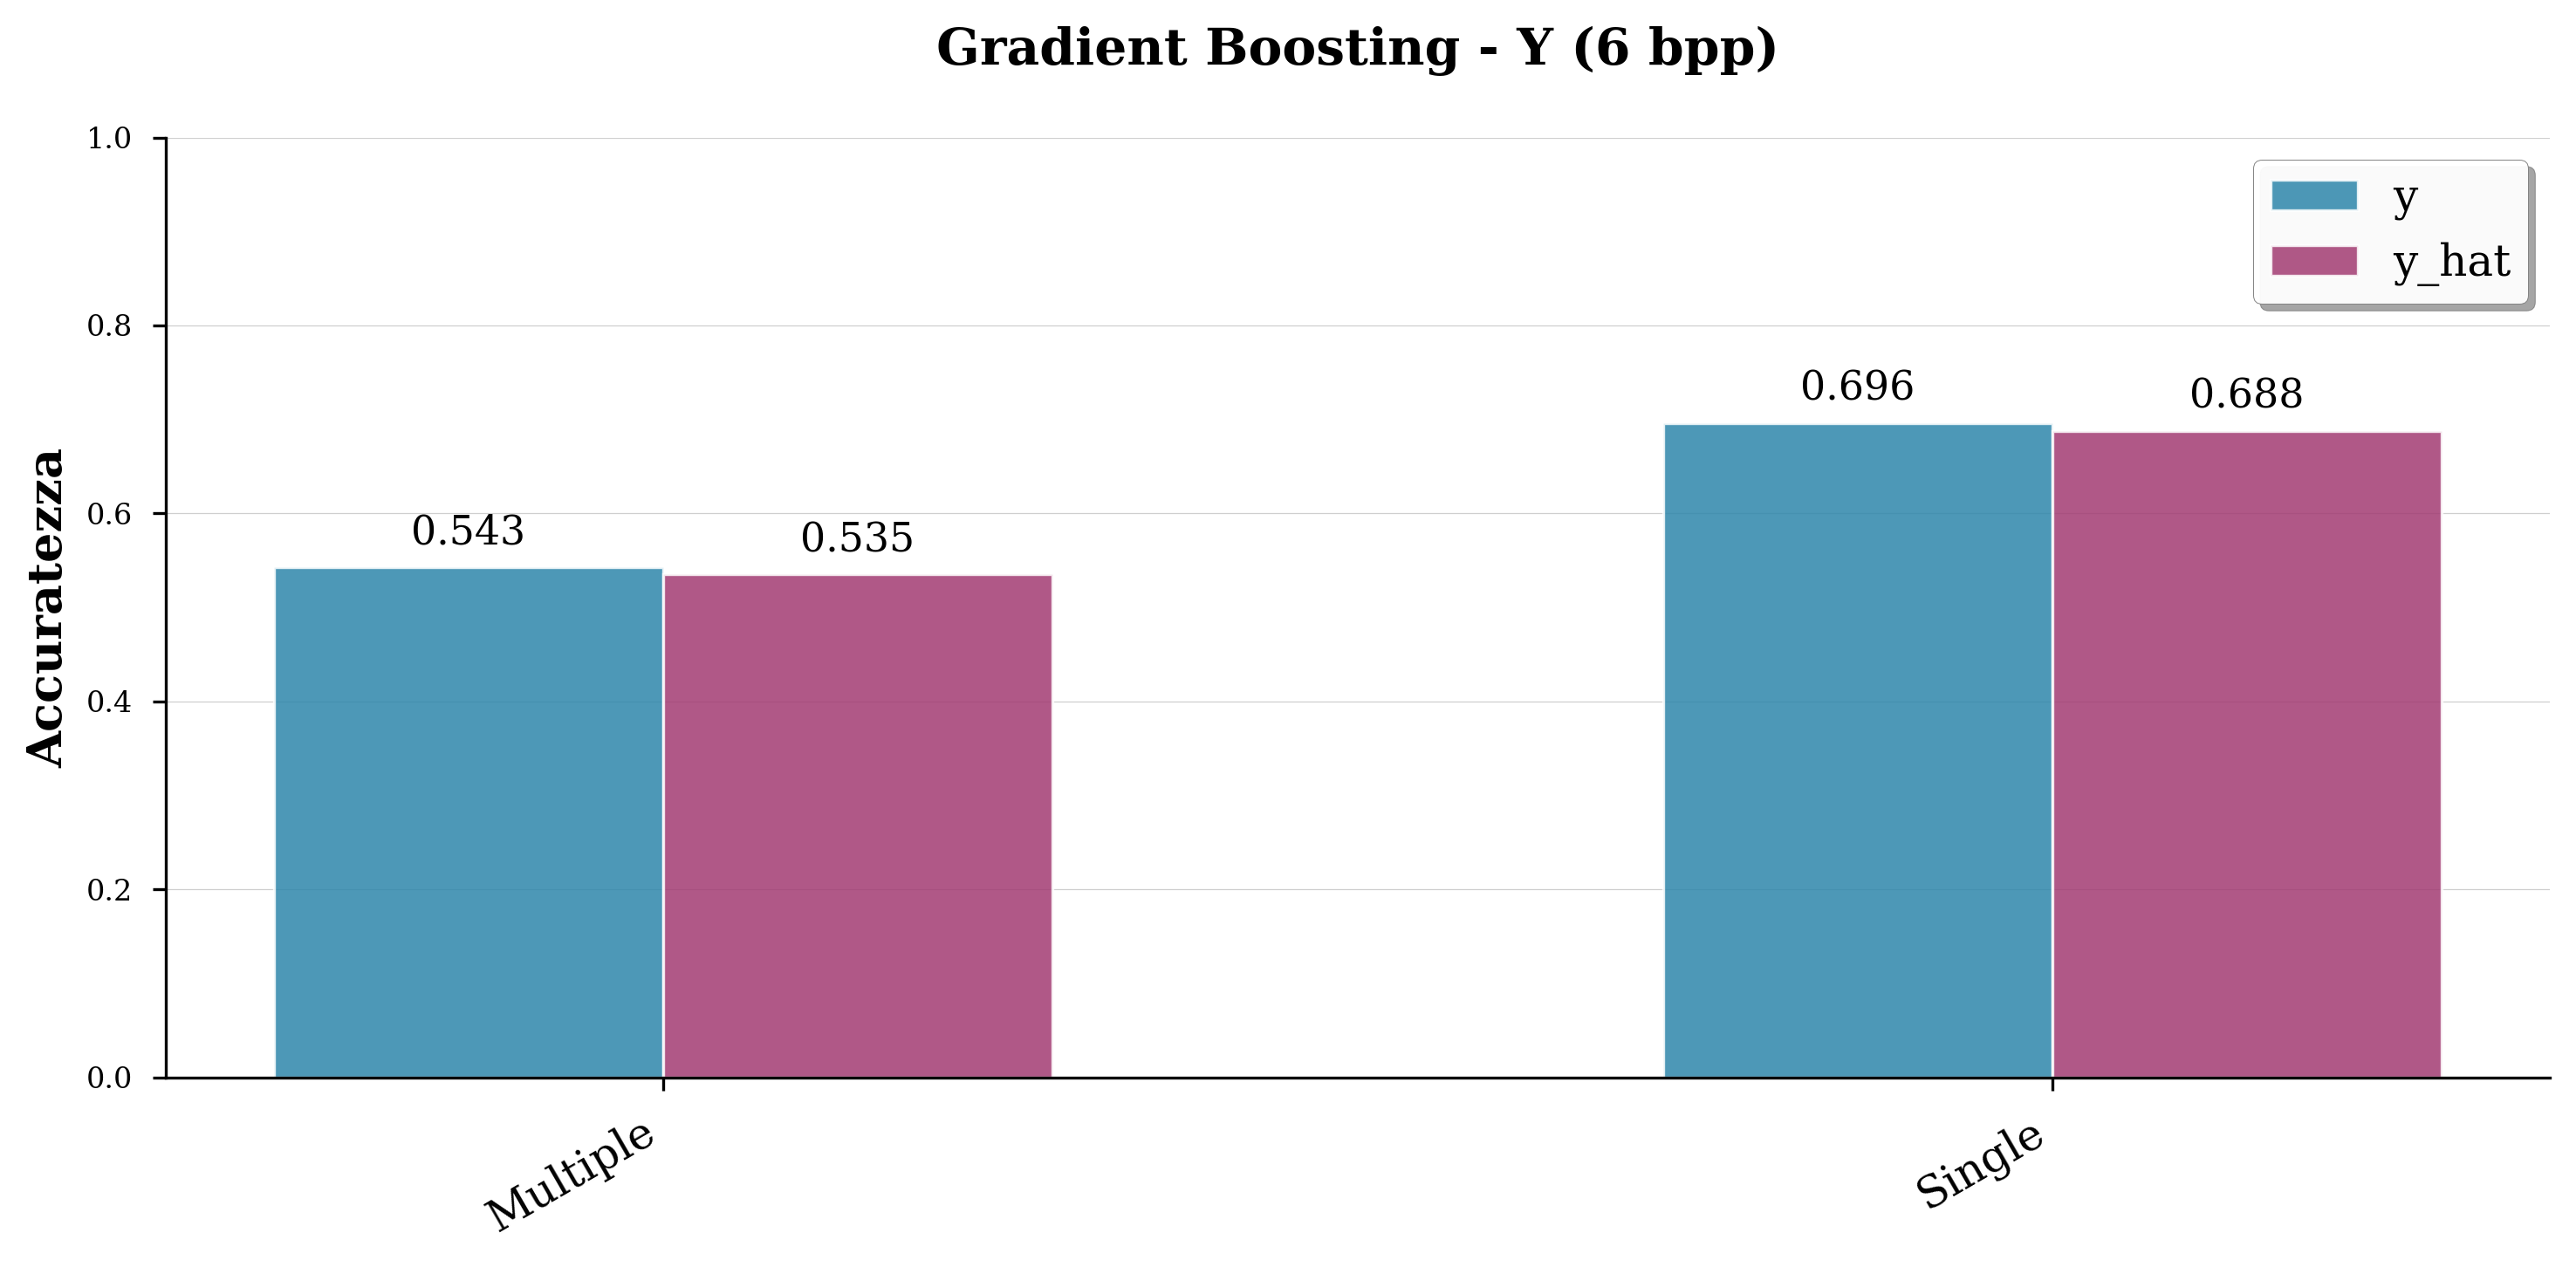
\includegraphics[width=0.8\textwidth]{figures/GB_Y_6bpp_improved.png}\\[0.5cm]
    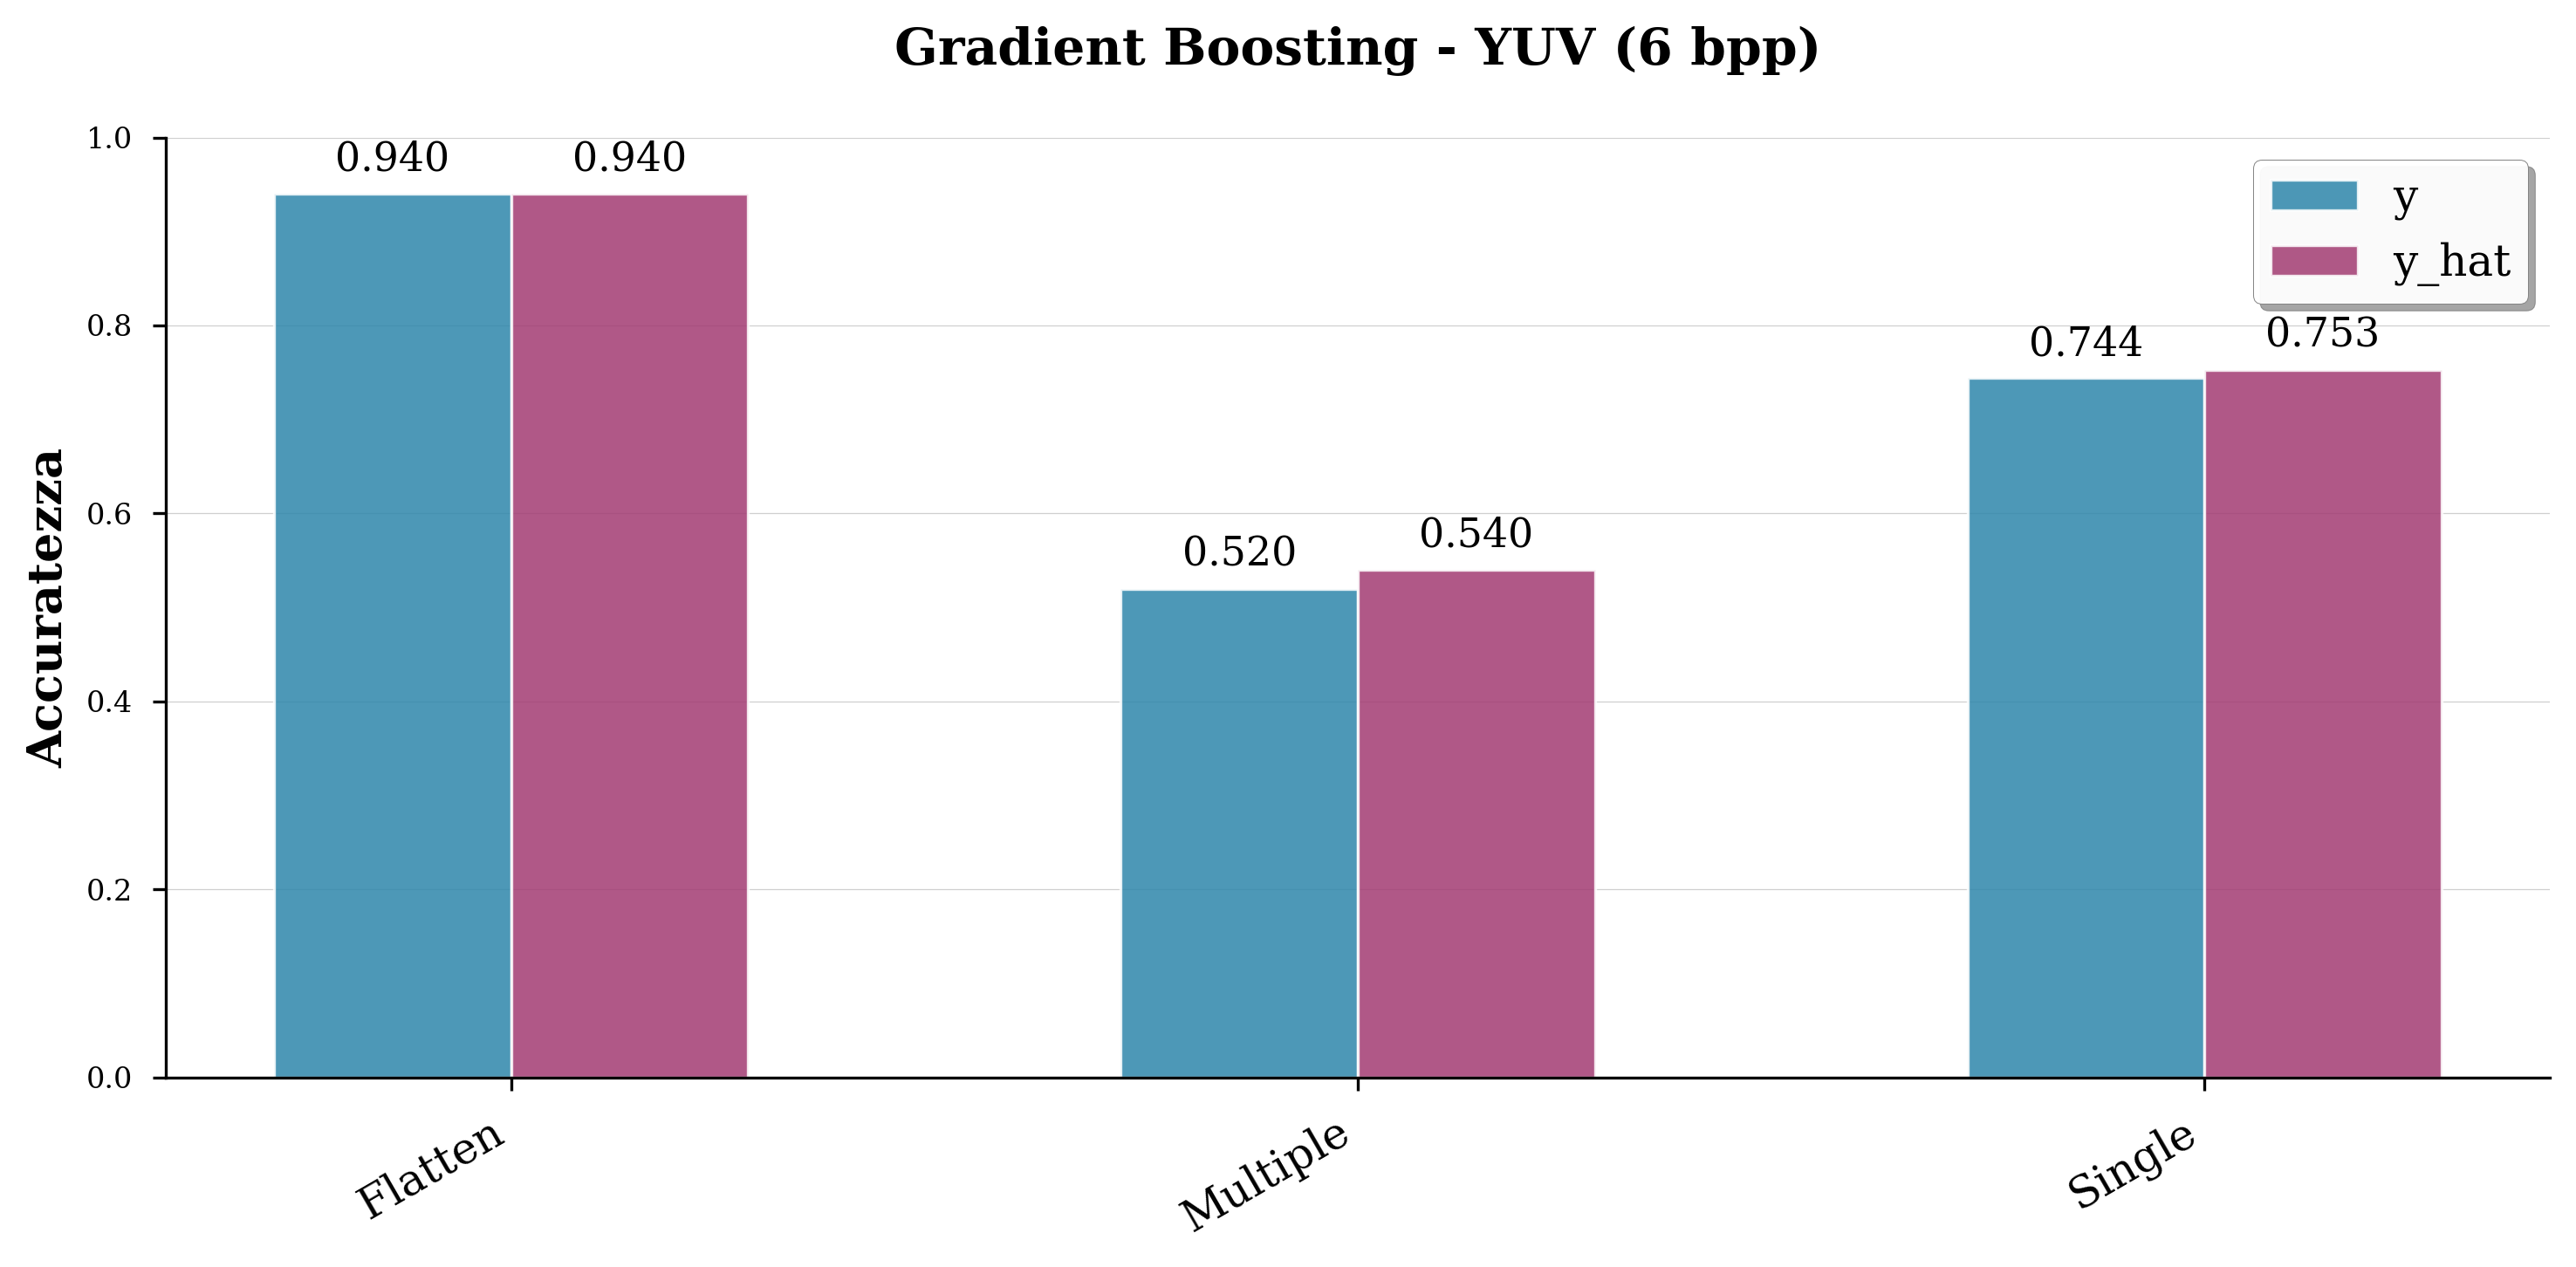
\includegraphics[width=0.8\textwidth]{figures/GB_YUV_6bpp_improved.png}
    \caption{Esempi di diagrammi a barre riguardanti performance di Gradient Boosting}
    \label{fig:GB_YUV_plots}
\end{figure}
Dai risultati osservati si nota un comportamento simile a quello del Random Forest, ottenendo migliori prestazioni con il metodo flatten e l'uso di tutte e tre le componenti YUV.
Nella figura \ref{fig:GB_YUV_confusion} sono riportate le matrici di confusione per le configurazioni che hanno ottenuto migliori prestazioni.
\begin{figure}[H]
    \centering
    \begin{subfigure}[b]{0.7\textwidth}
        \centering
        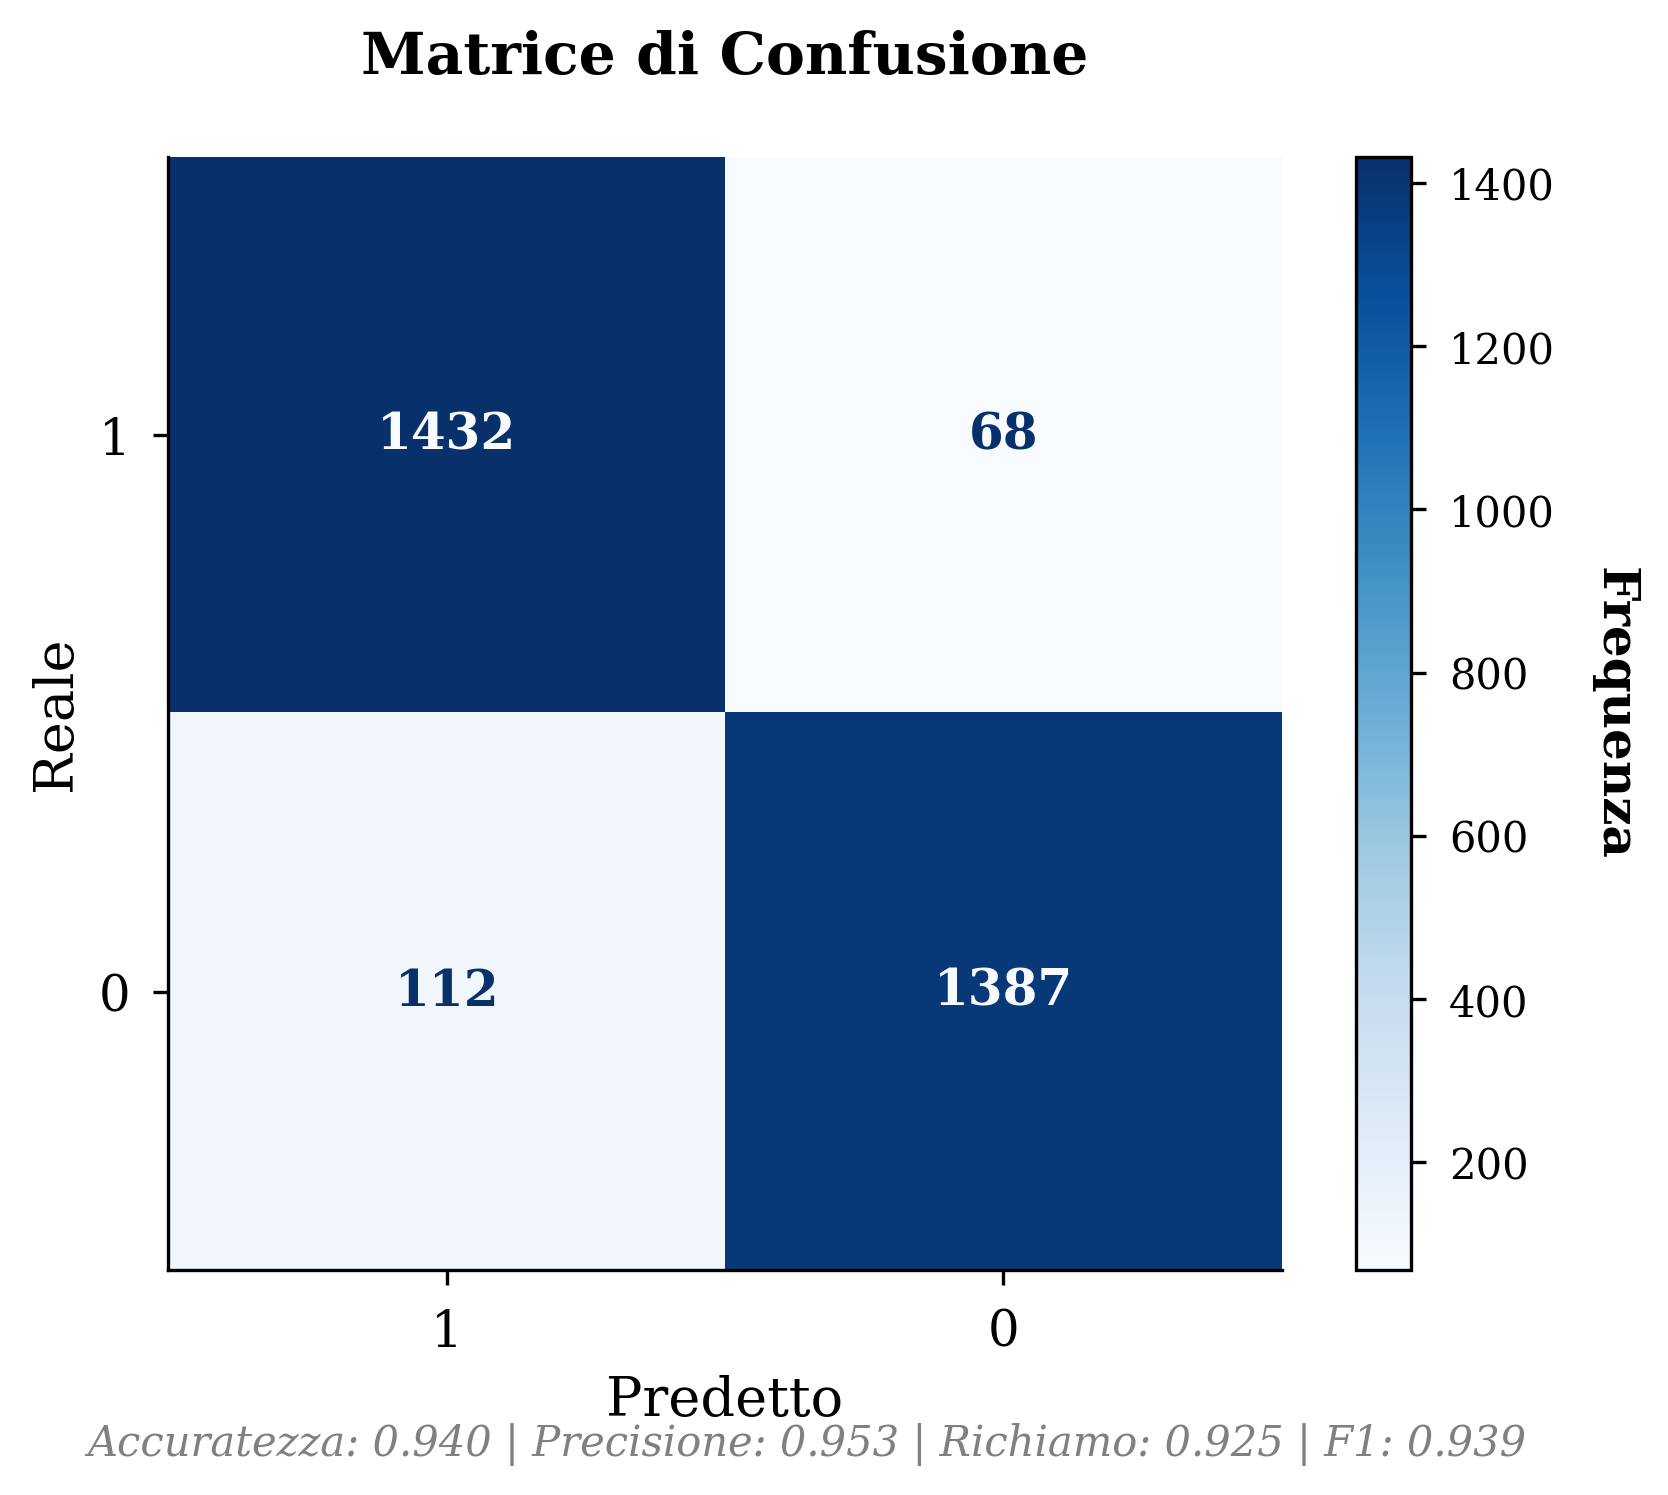
\includegraphics[width=\textwidth]{figures/confusion_matrix_YUV_flatten_GB.png}
        \caption{Metodo flatten}
    \end{subfigure}
    \hfill
    \begin{subfigure}[b]{0.7\textwidth}
        \centering
        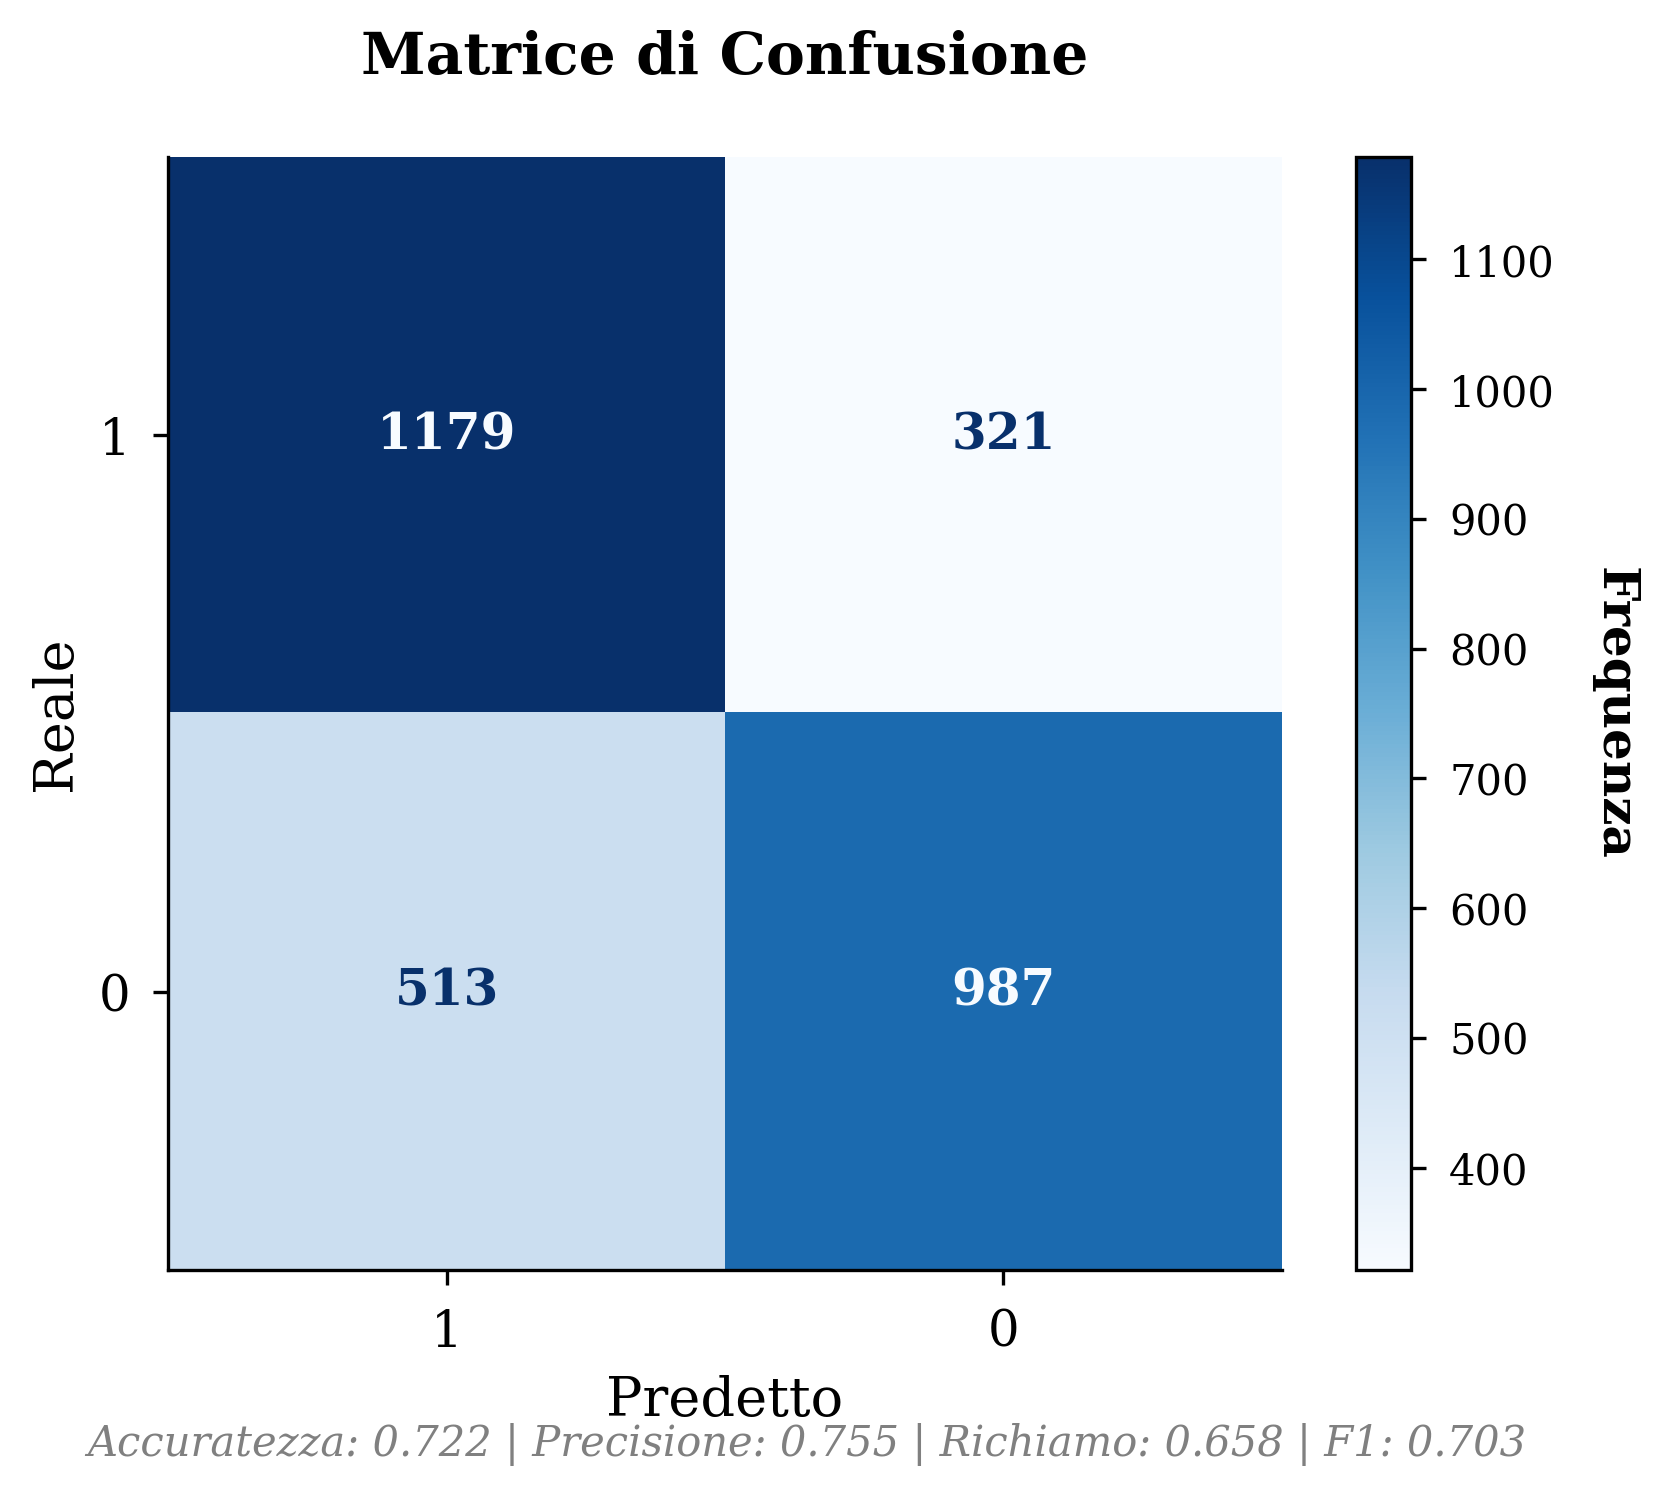
\includegraphics[width=\textwidth]{figures/confusion_matrix_YUV_single_GB.png}
        \caption{Metodo single patch}
    \end{subfigure}
    \caption{Matrici di confusione per Gradient Boosting allenato su YUV con due approcci diversi.}
    \label{fig:GB_YUV_confusion}
\end{figure}
\subsection{Confronto tra classificatori}
Nei diagrammi presenti nelle figure \ref{fig:GB_RF_Y_comparison} e \ref{fig:GB_RF_YUV_comparison} viene mostrato il confronto diretto tra le prestazioni dei due classificatori a diversi livelli di compressione.
\begin{figure}[H]
    \centering
    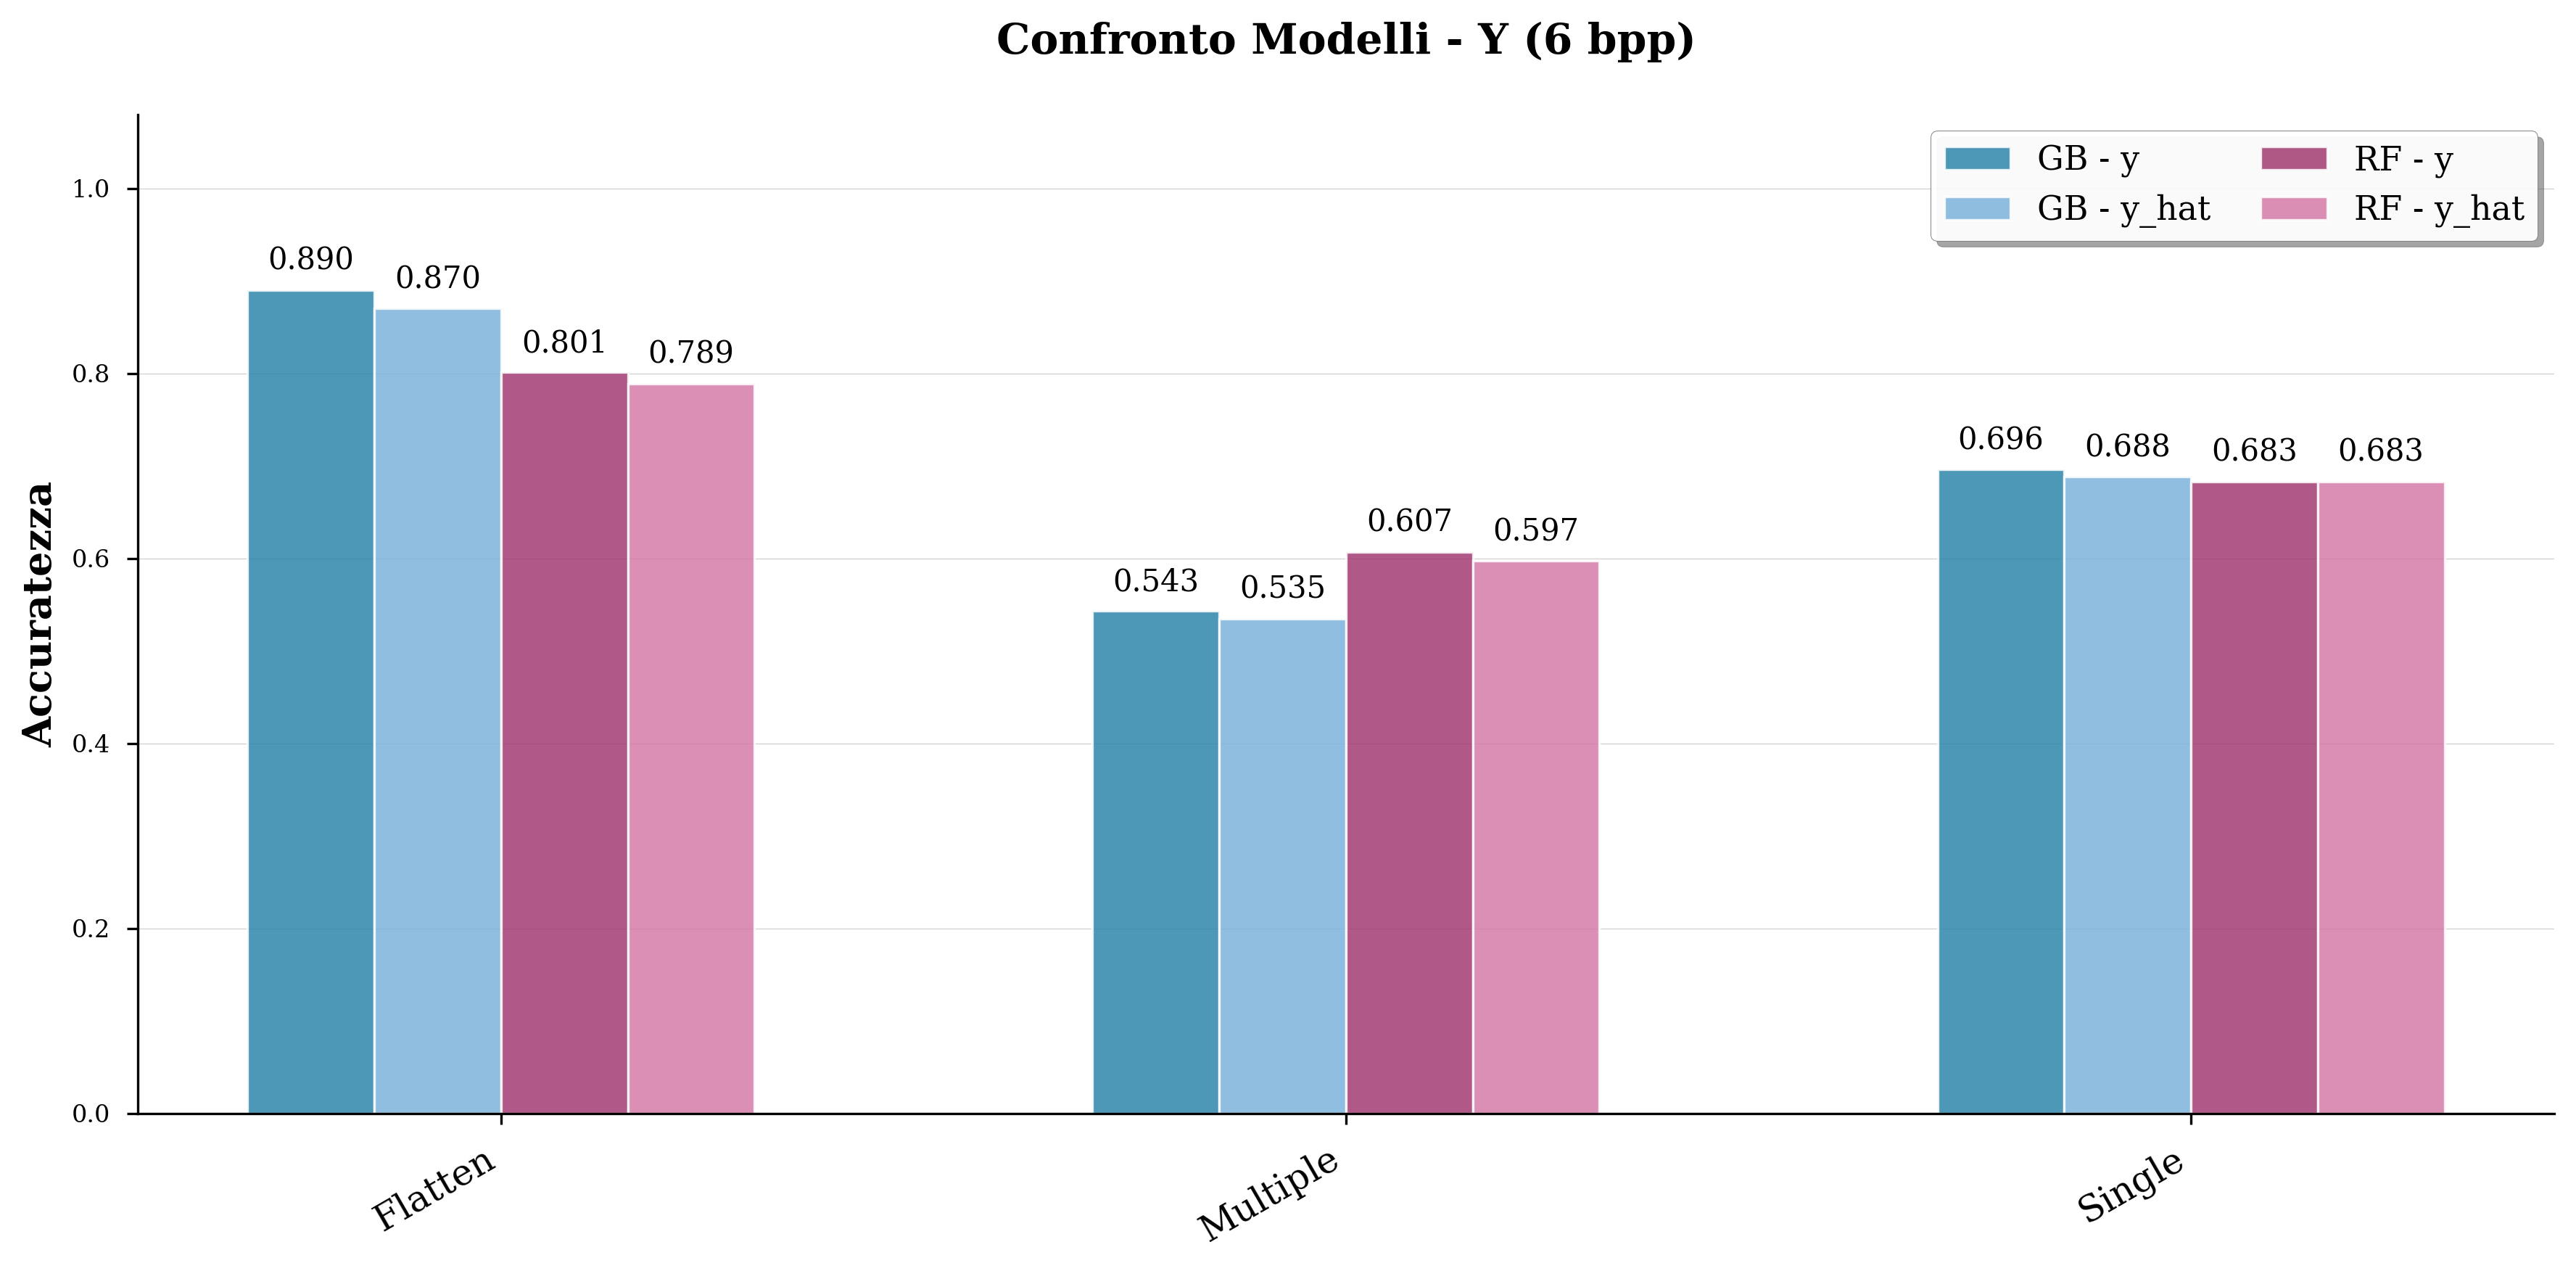
\includegraphics[width=\textwidth]{figures/Compare_GB_RF_Y_6bpp_improved.png}
    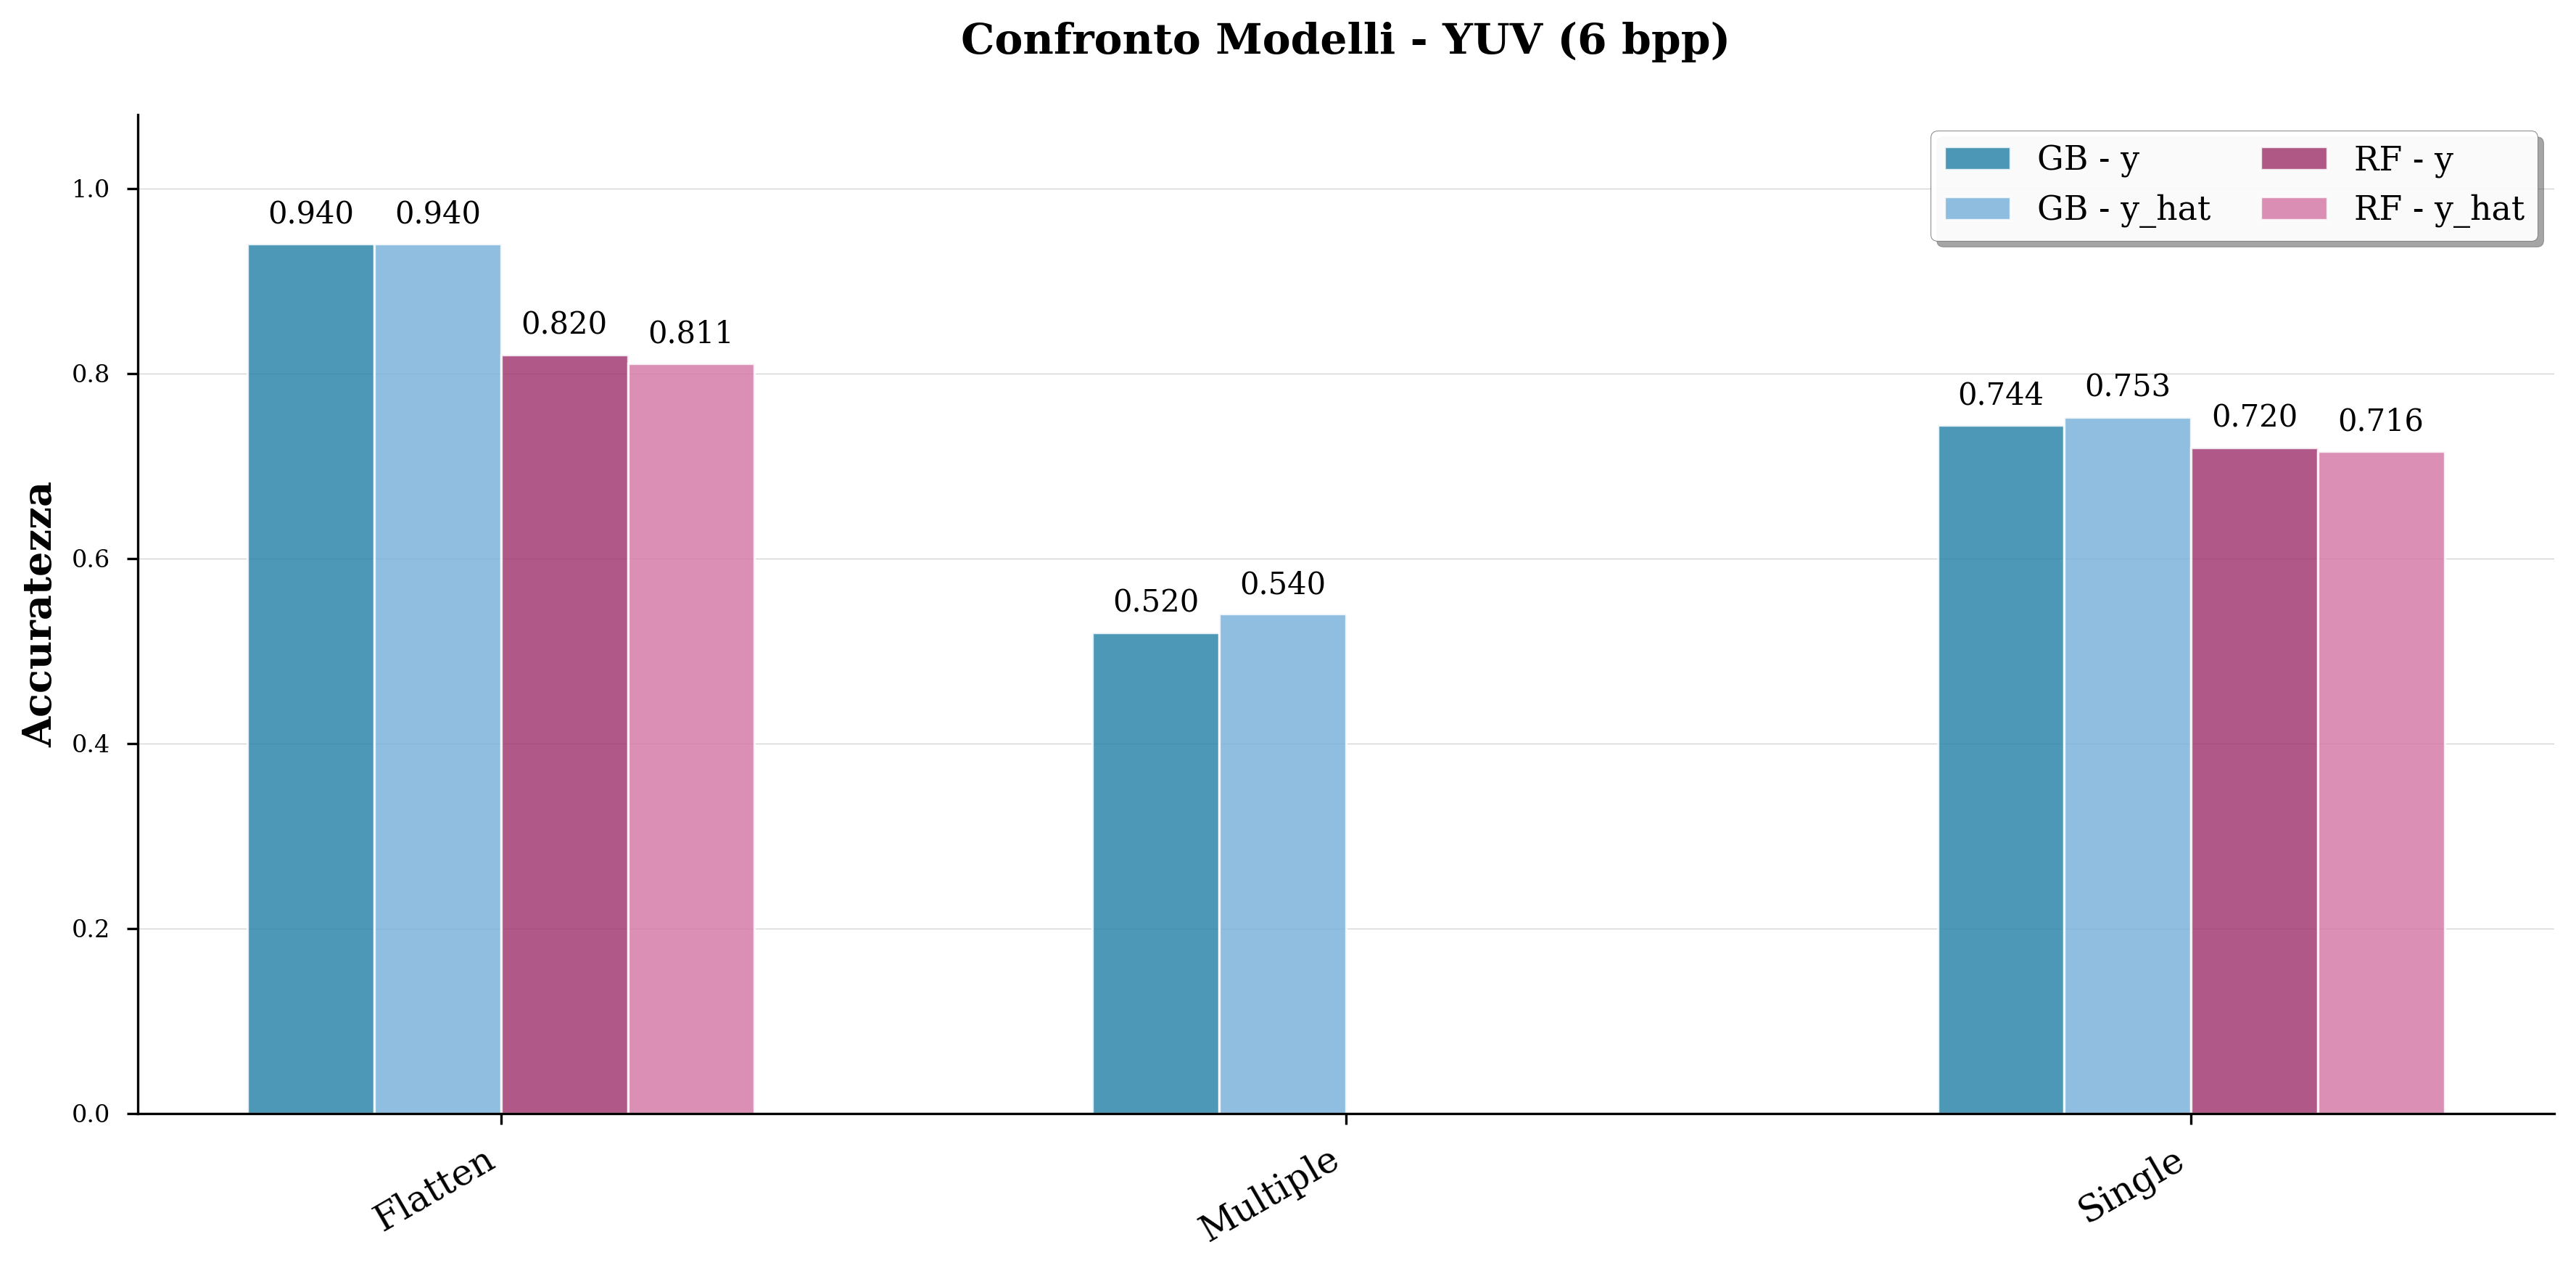
\includegraphics[width=\textwidth]{figures/Compare_GB_RF_YUV_6bpp_improved.png}
    \caption{Confronto tra Gradient Boosting e Random Forest a 6bpp.}
    \label{fig:GB_RF_Y_comparison}
\end{figure}

\begin{figure}[H]
    \centering
    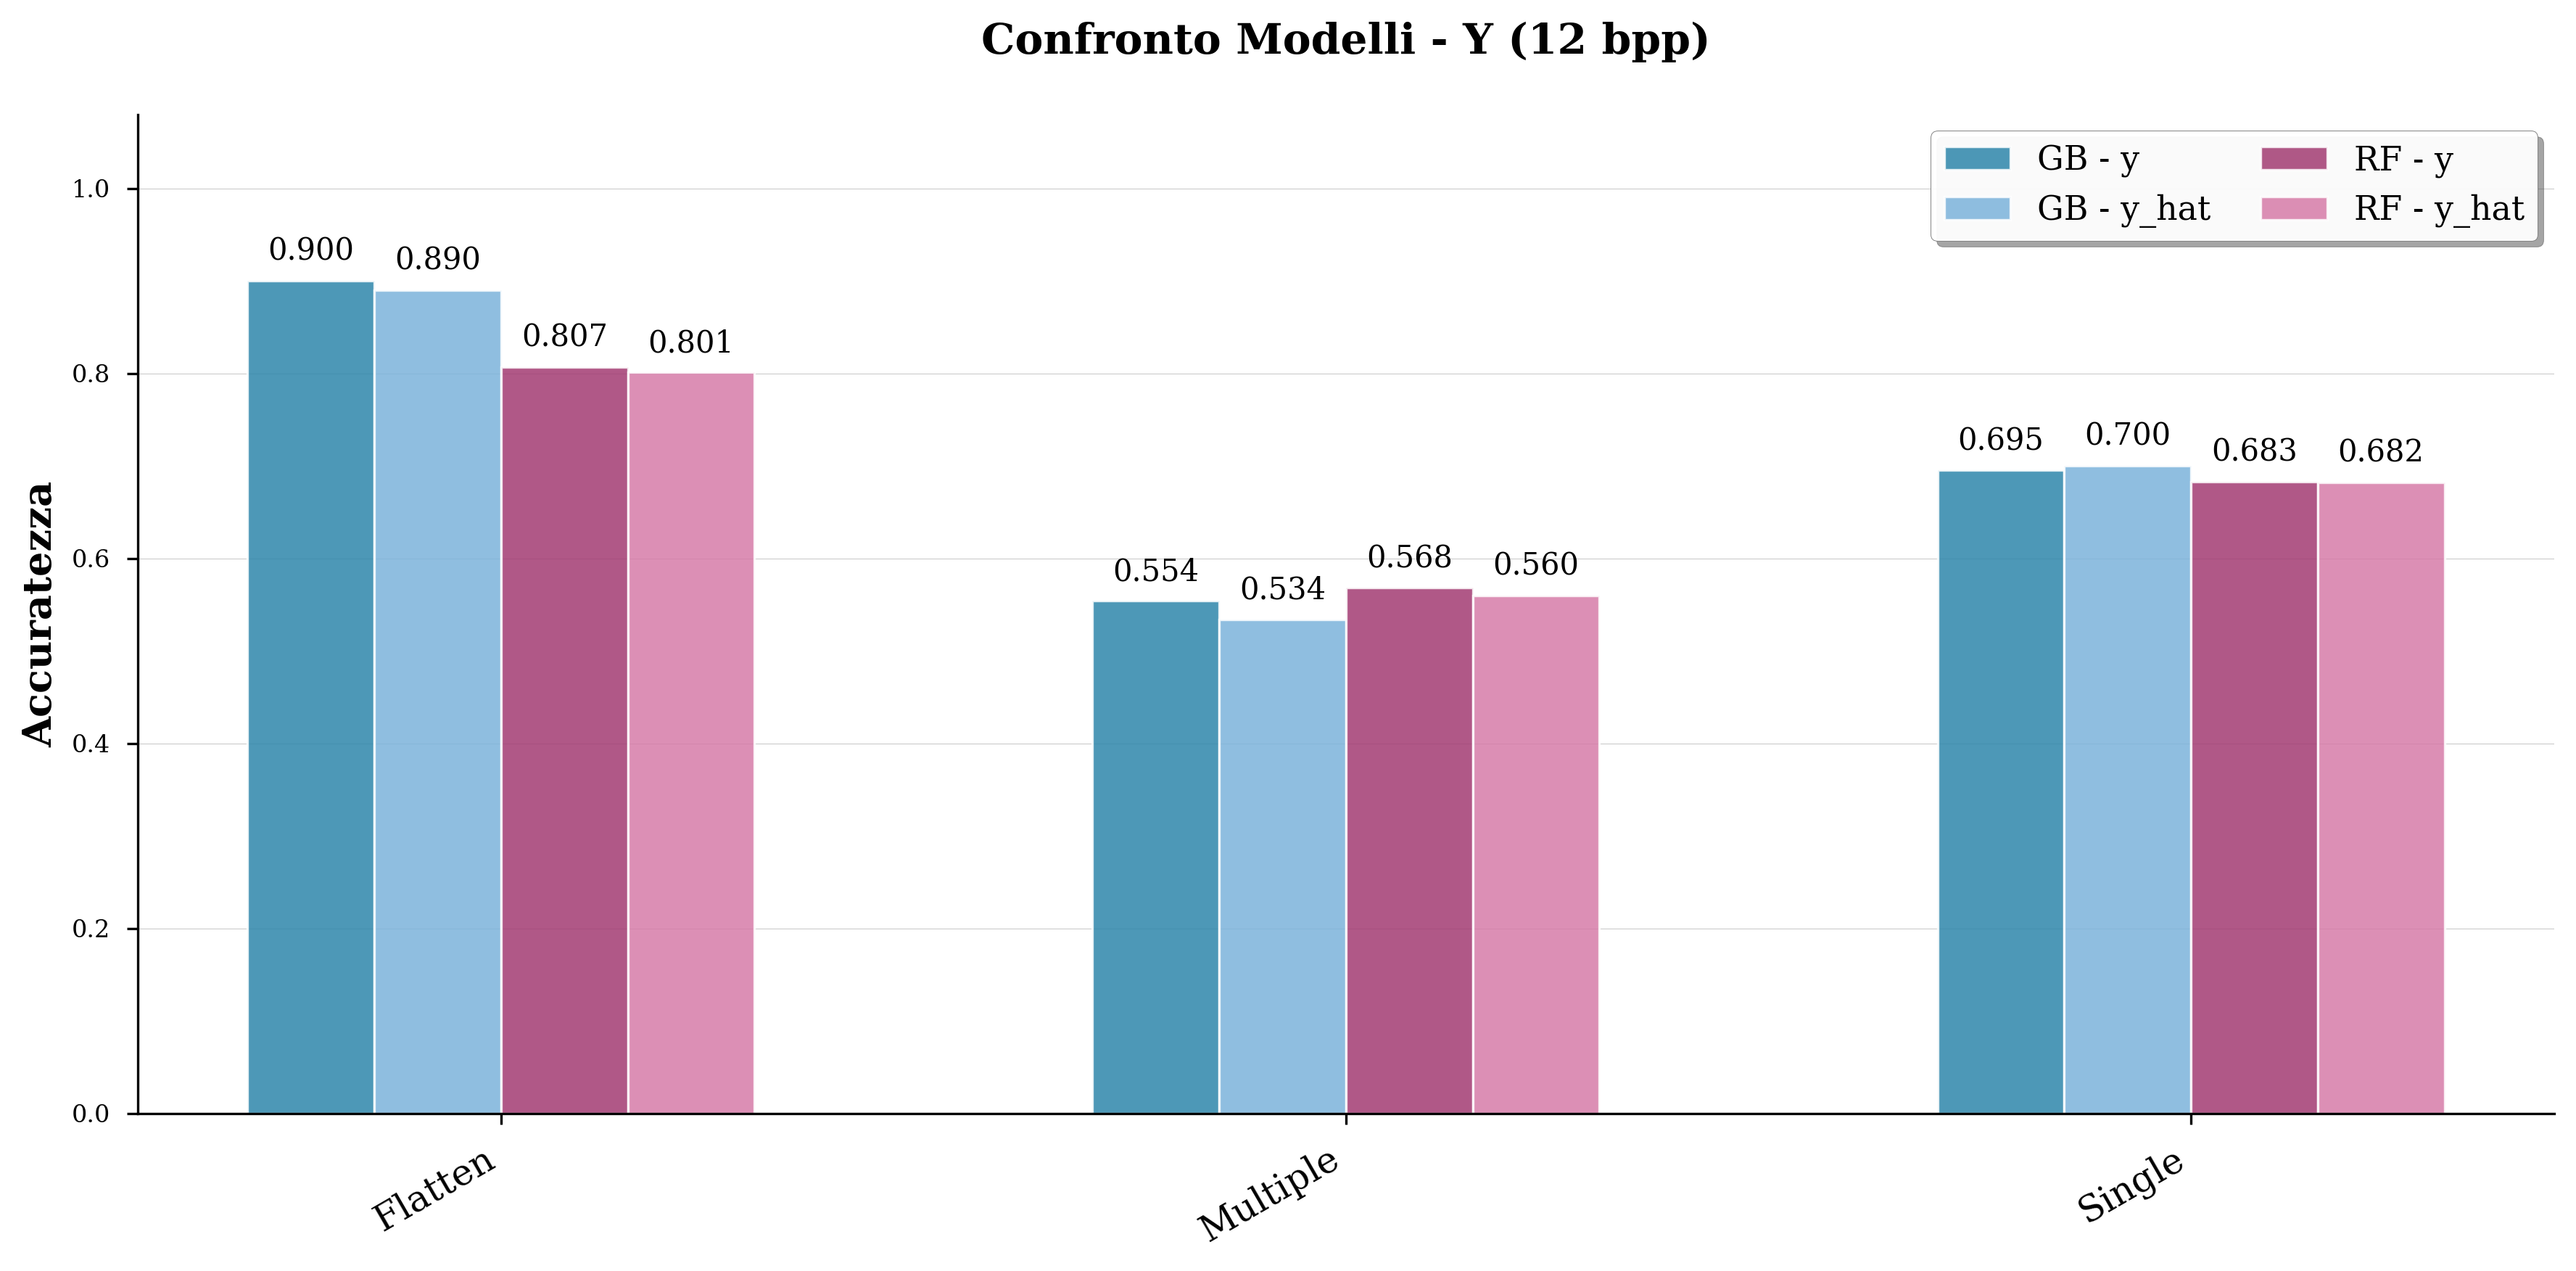
\includegraphics[width=\textwidth]{figures/Compare_GB_RF_Y_12bpp_improved.png}
    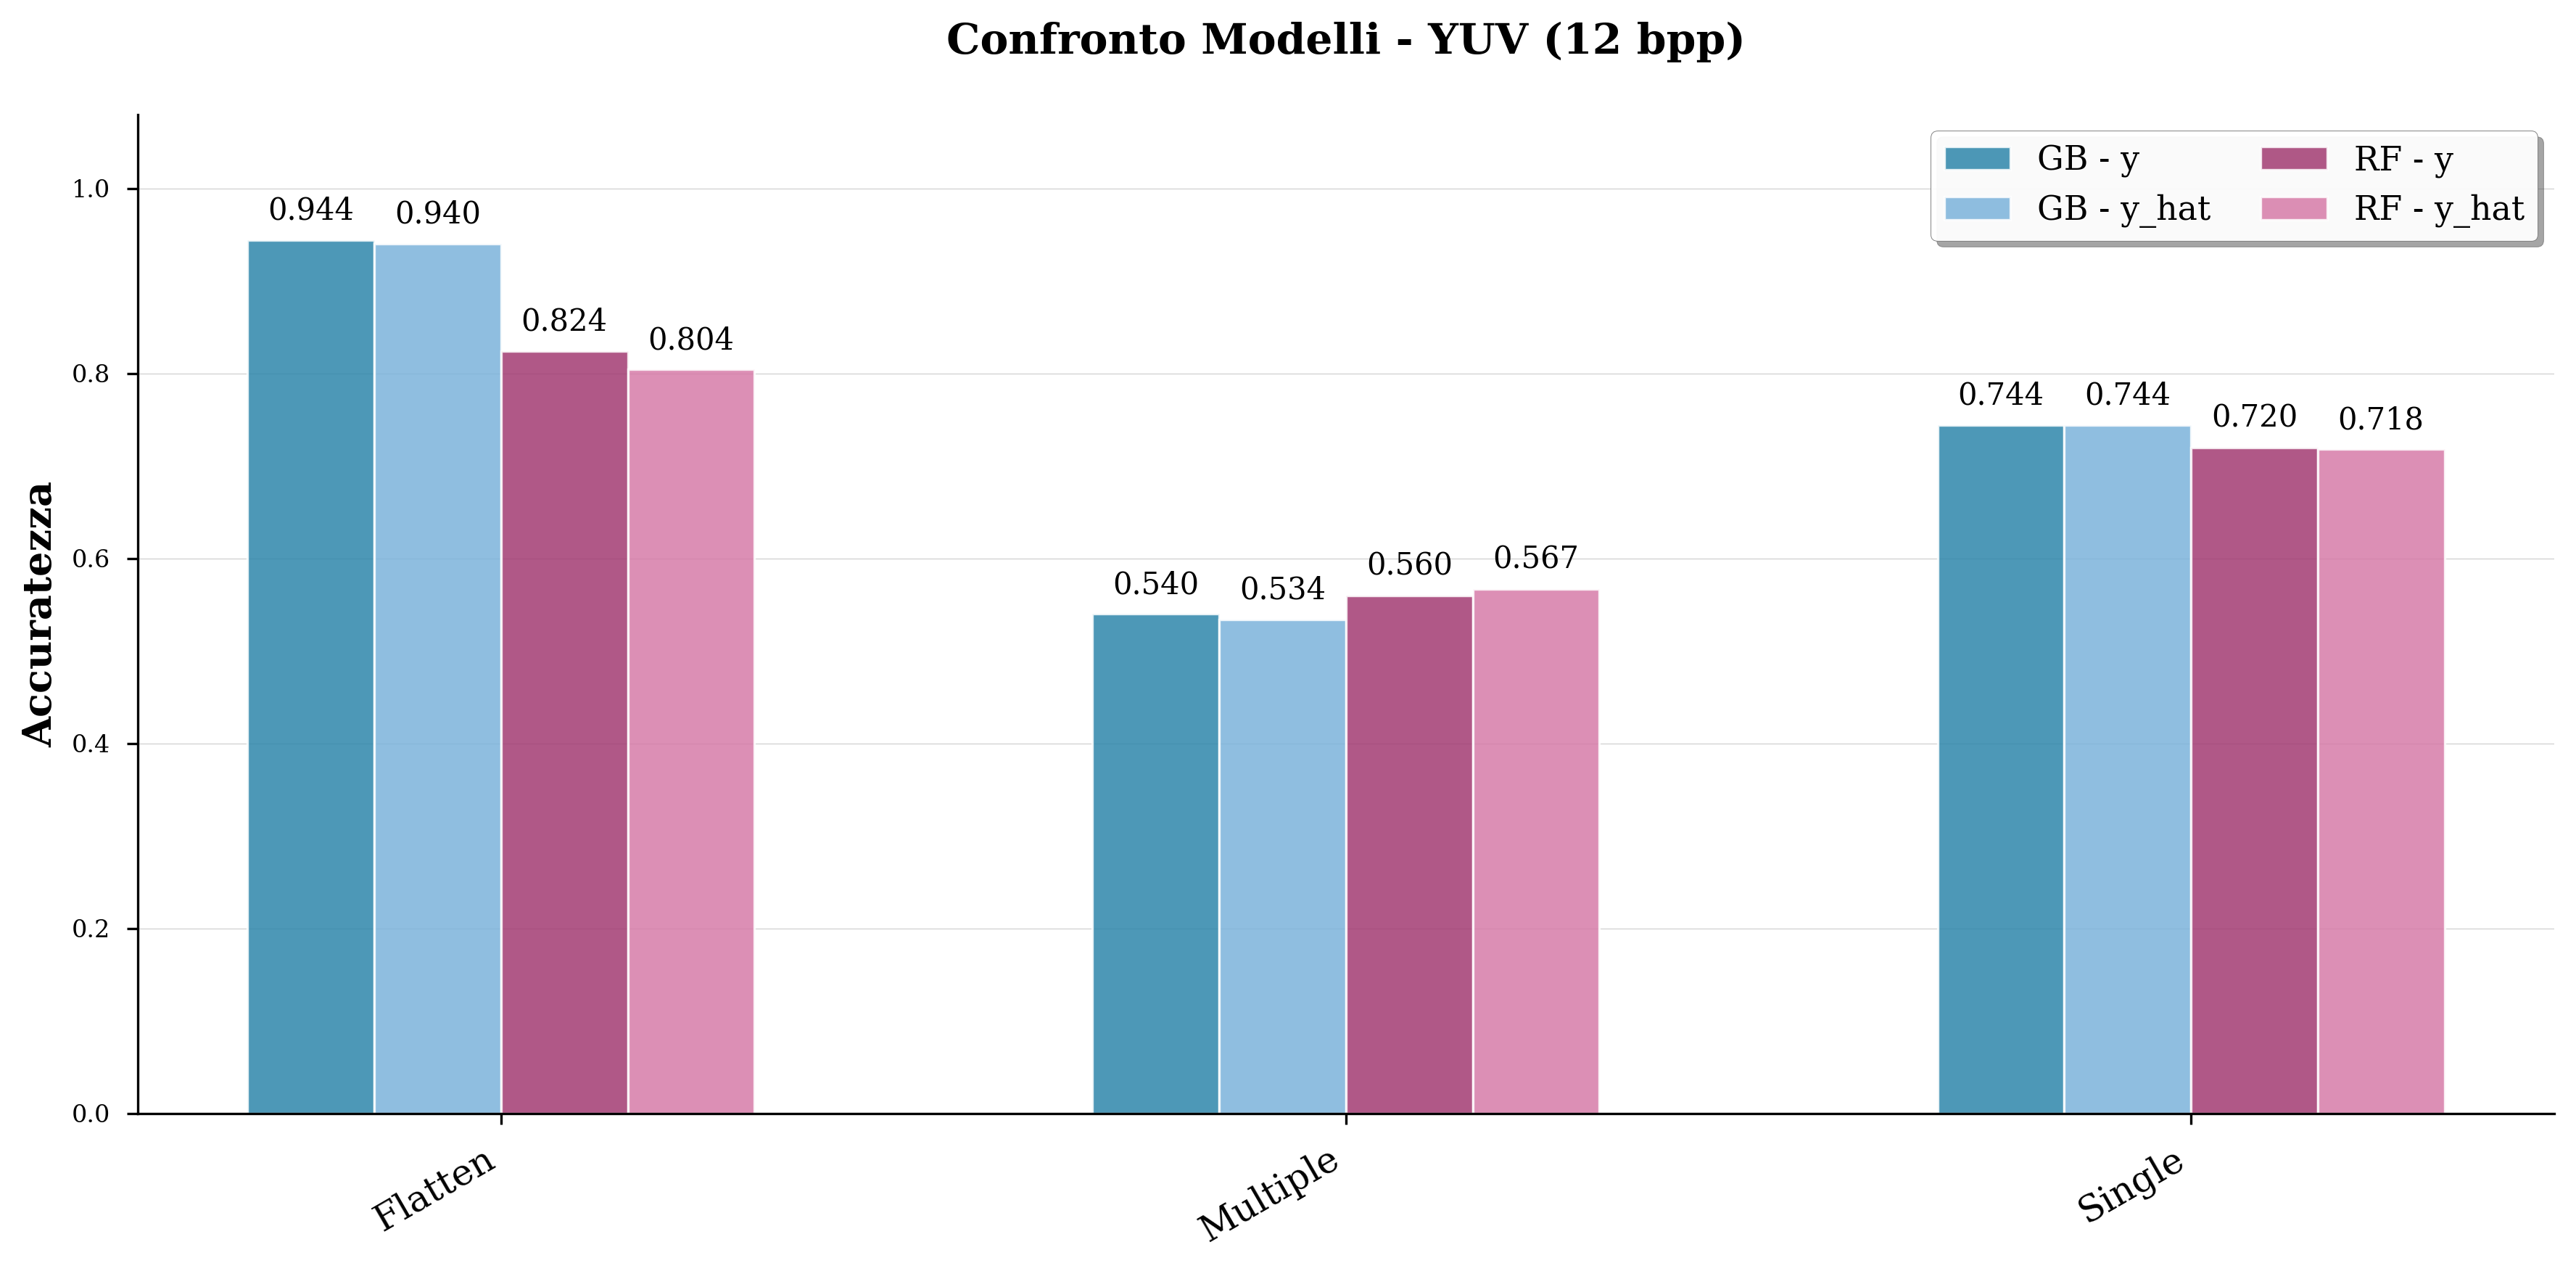
\includegraphics[width=\textwidth]{figures/Compare_GB_RF_YUV_12bpp_improved.png}
    \caption{Confronto tra Gradient Boosting e Random Forest a 12 bpp.}
    \label{fig:GB_RF_YUV_comparison}
\end{figure}
Dall'analisi dei risultati si può notare come l'accuratezza non subisca grandi varianzioni ai diversi livelli di compressione scelti, mentre è evidente la differenza tra le performance dei modelli allenati esclusivamente sulla componente di luminanza e quelli allenati anche usando la crominanza. Questo è ragionevole in quanto la differenza risiede nel fatto che nel secondo caso il classificatore ha più informazioni a disposizione da sfruttare nella classificazione.\\
La miglior accuratezza in presenza di più informazioni viene confermata anche dai risultati ottenuti con i diversi metodi di preprocessing: il metodo flatten, che permette di allenare i modelli su tutti i valori disponibili delle rappresentazioni latenti originali, ottiene risultati migliori in tutti i casi. Questo però non avviene senza cosi, infatti con l'aumento della dimensionalità dei campioni per allenare i modelli, riportati nella tabella \ref{tab:preprocessing_methods}, corrisponde ad un aumento nei tempi di addestramento e una maggior necessità di risorse computazionali. Nella tabella \ref{tab:training_times} sono riportati i tempi di addestramento per ogni combinazione di fattori.
\begin{table}[H]
\centering
\caption{Tempi di addestramento per dataset di $30.000$ immagini}\label{tab:training_times}
\begin{tabular}{l c c}
\toprule
Modello & Preprocessing & Tempo di addestramento \\
\midrule
RF &      single &  $\sim$3min \\
RF &    multiple &  $\sim$20min\\
RF &      flatten &  $\sim$1h45min\\
\midrule
GB &      single &  $\sim$2min \\
GB &    multiple &  $\sim$15min \\
GB &      flatten &  $\sim$1h \\
\bottomrule
\end{tabular}
\end{table}
Il metodo di single patch risulta essere il miglior compromesso tra accuratezza e tempi di addestramento, ma ha il problema della forte dipendenza dalla posizione della patch estratta. Il metodo multiple patches ha ottenuto risultati peggiori, ma potrebbe essere utilizzato in casi dove non sono disponibili molti campioni di addestramento, permettendo di aumentare la cardinalità del dataset come mostrato nella tabella \ref{tab:preprocessing_methods}.\\
Inoltre, osservando le tabelle \ref{fig:GB_RF_Y_comparison} e \ref{fig:GB_RF_YUV_comparison} si può notare come Gradient Boosting ottenga un'accuratezza in generale più alta rispetto alla variante Random Forest, dovuta dalla diversa modalità con il quale vengono costruiti gli alberi di decisione di base.\\